\chapter{Probabilistic rules}
\label{chap:rules}

This chapter spells out the dialogue modelling approach developed in this thesis.  The previous chapter described how dialogue could be modelled in a probabilistic manner, and demonstrated how graphical models can help reduce the complexity of probability and utility models by exploiting independence properties between variables. But despite these attractive properties, graphical models still suffer from severe scalability problems when faced with complex dialogue domains.  Dependent variables can lead to an rapid increase in the number of parameters associated with the model. Alas, only limited amounts of training data are available for most dialogue domains.  Estimating the model parameters in such setting is therefore a particularly challenging task. 

To address this issue, we introduce in this chapter the notion of \textit{probabilistic rules}, which are structured mappings between conditions and  (parametrised) effects.  These rules function as \textit{high-level templates} for the construction of a dynamic decision network.  The key advantage of such structured modelling approach is the drastic reduction of the number of parameters compared to traditional representations.  We also argue that these expressive representations are particularly well suited to encode the probability and utility models used in dialogue management, where substantial amounts of expert knowledge can be leveraged to structure the relationships between variables. 

The chapter is divided in six sections:  Section \ref{sec:rmotivation} demonstrates in general terms how structural assumptions can be used to refine the representation of probabilistic models. Section \ref{sec:formalisation} show such structural assumptions can be practically encoded with probabilistic rules.  We formally define these rules in terms of conditions and effects and provide some concrete examples of rules for dialogue management.  Section \ref{sec:ruleinstantiation} connects these definitions to the graphical models described in the previous chapter by showing how probabilistic rules are practically instantiated into a graphical model.  Finally, Section \ref{sec:amodelling} addresses some advanced modelling issues and Section \ref{sec:relatedwork} relates the approach to previous work.


\section{Structural leverage}
\label{sec:rmotivation}

The starting point of our approach is the observation that the probability and utility models used in dialogue management often exhibit a fair amount of \textit{internal structure}.  
We have already discussed in the previous chapter one simple instance of this internal structure: factored representations based on conditional independences. However, the internal structure of dialogue domains does not limit itself to these basic independence assumptions, and much can be gained in exploiting additional structural properties. 

%If two sets of random variables $\mathbf{X}$ and $\mathbf{Y}$ are conditionally independent given $\mathbf{Z}$, we can rewrite the probability distribution $P(\mathbf{X}, \mathbf{Y} \, | \, \mathbf{Z})$ as $P(\mathbf{X} \, | \, \mathbf{Z}) (\mathbf{Y} \, | \, \mathbf{Z}) $.  


\subsubsection*{Latent variables}
 
The number of parameters required to estimate the distributions of a graphical model can often be reduced by introducing \textit{latent variables} (i.e. unobserved or hidden variables) as intermediaries between the source and target variables. Indeed, many application domains are often best explained by the combination of a small number of distinct factors or influences, each encoded by a separate random variable and associated with a subset of input and output variables. Theses variables are usually never observed directly but contribute to structuring the model.\footnote{The use of layered computational models is one of the most active research topic in many areas of artificial intelligence and machine learning, and form in particular the foundations of deep learning approaches \citep{Bengio:2009}.} In the particular case of medical diagnosis, the relation between predisposing factors and observed symptoms are for instance preferably described by postulating an intermediary layer of variables -- possible diseases -- that mediate between the predisposing factors and the observed symptoms.  Figure \ref{fig:latentvariables} illustrates how latent variables can be exploited to provide an additional layer of abstraction within a graphical model.

 \begin{figure}[h]
\centering
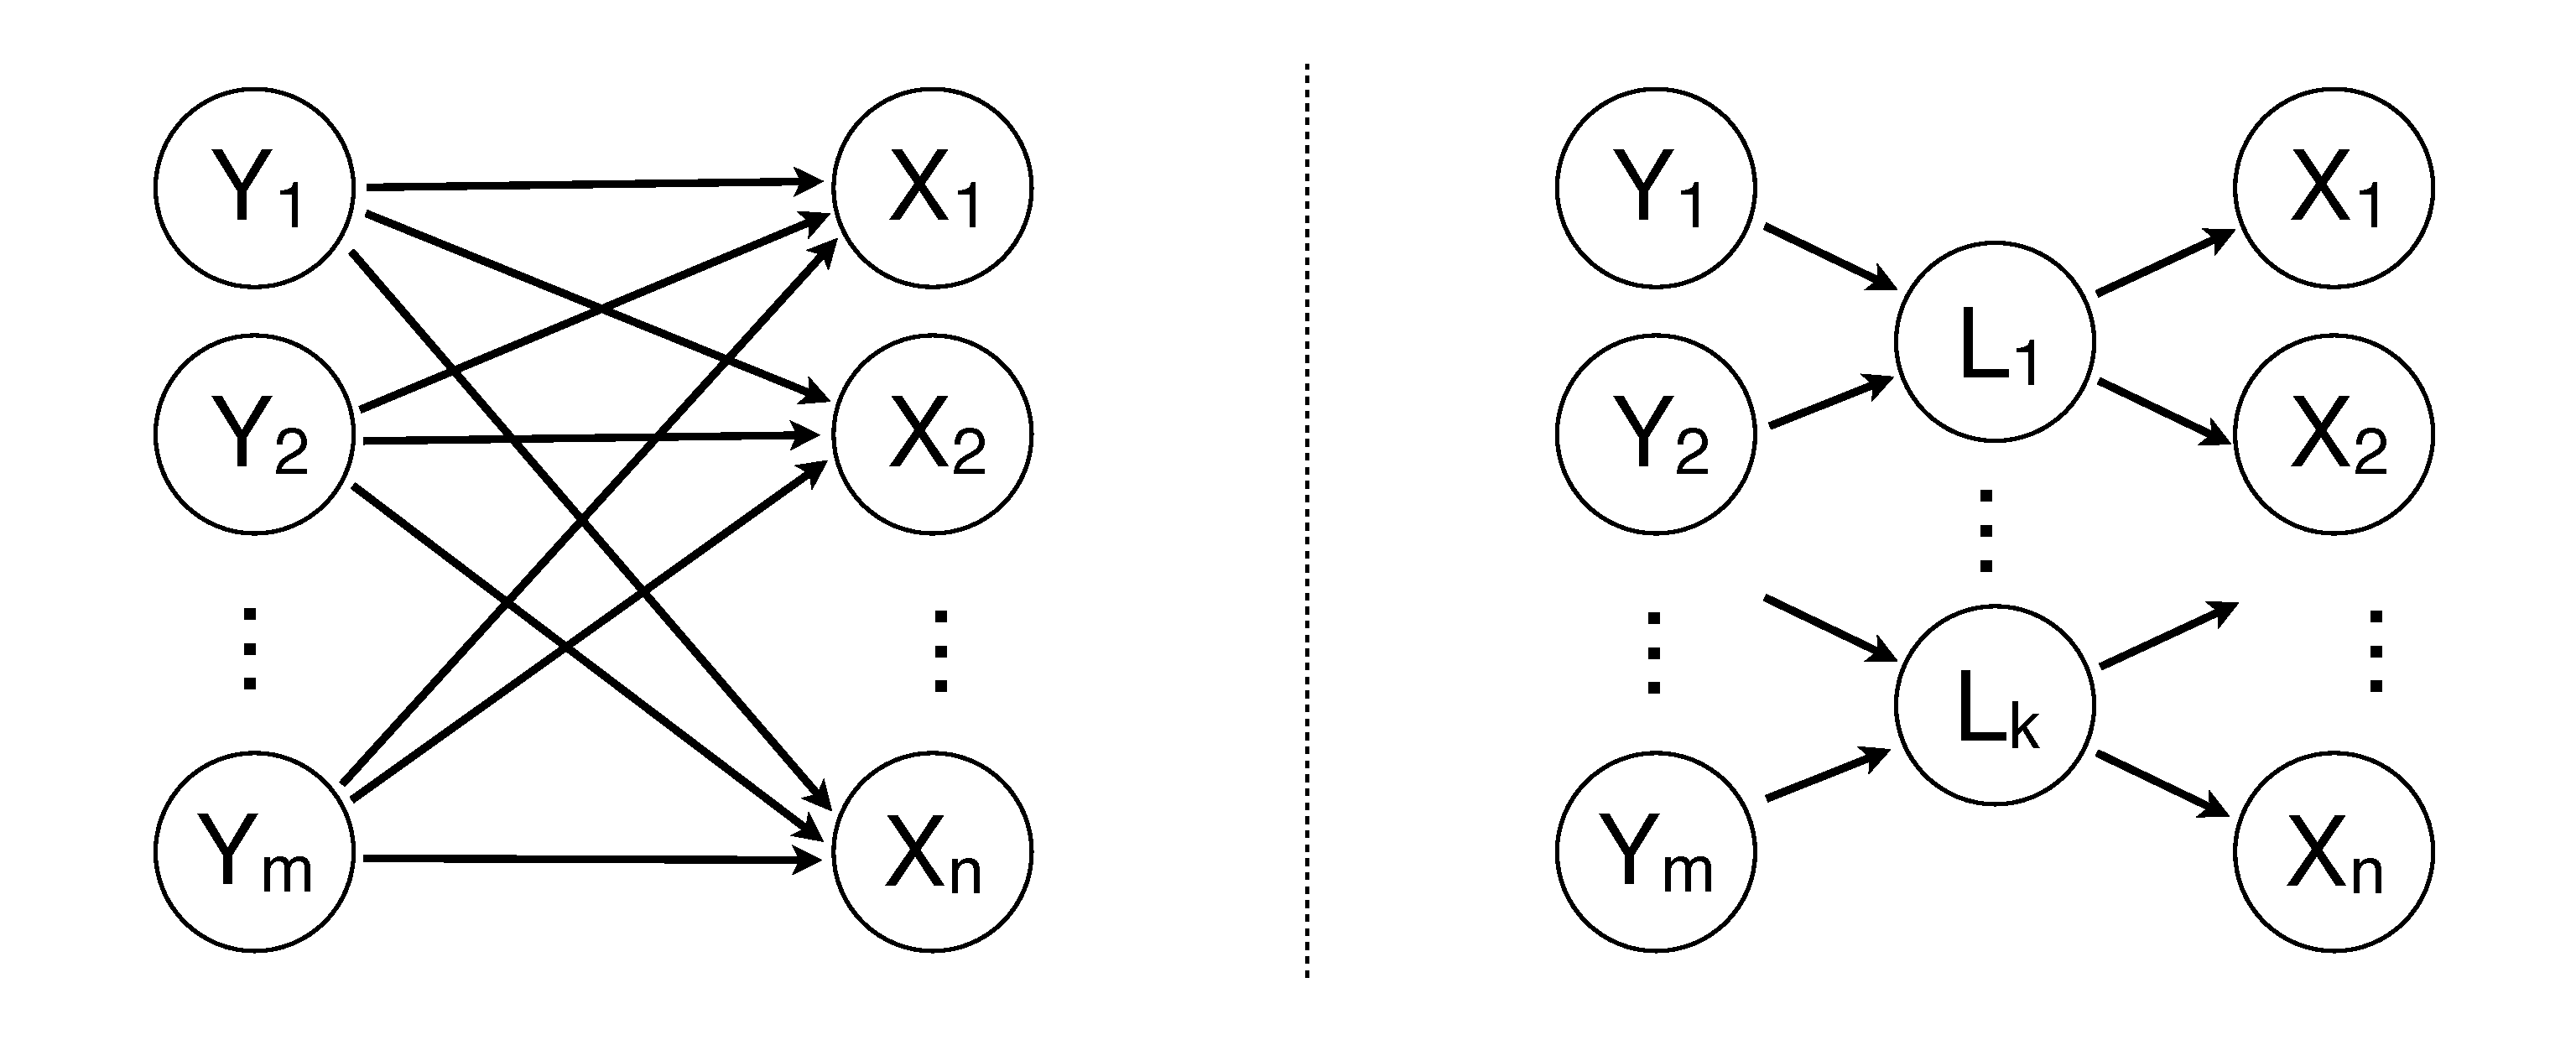
\includegraphics[scale=0.25]{imgs/latentvariables.pdf}
\caption{Comparison between a model that directly maps variables $\mathbf{Y}$ to $\mathbf{X}$ (left side) and one relying on latent variables $\mathbf{L}$ to serve as intermediaries (right side).}
\label{fig:latentvariables}
\end{figure}

Dialogue models can often benefit from introduction of such latent variables. The transition function can in particular be modelled in terms of a limited number of latent variables, each responsible for capturing specific aspects of the interaction dynamics. 

\subsubsection*{Partitioning}

A random variable $X$ with parent variables $Y_1,...Y_m$ must specify a separate probability distribution for every possible assignment of values for the parent variables. In other words, the number of parameters required to specify the distribution $P(X \, | \, Y_1,..., Y_m)$ is exponential in the number of parents $m$. Fortunately, the values of these parents variables can be grouped into \textit{partitions} yielding similar outcomes for $X$. One can therefore directly define the conditional probability distributions on these groups than on the full enumeration of combined values for the parent variables. Partitioning is an important abstraction mechanism to reduce the complexity of the model distributions and hence improve their ability to generalise to unseen examples. Utility distributions can also partition the values of their dependent variables in a similar way.  

Figure \ref{fig:partitioning} provides an example of such partitioning for the conditional probability distribution $P(\mathit{Fire} \, | \mathit{Weather}, \mathit{Rain})$.  The space of possible values for the parent variables is defined in this example as $Val(\mathit{Weather}) \times Val(\mathit{Rain})$ and contains 6 possible elements.  We can observe that this space can be defined in two partitions: $\mathit{Rain}\!=\mathit{true} \lor \mathit{Weather}\!\neq\mathit{hot}$ and $\mathit{Rain}\!=\mathit{false} \land \mathit{Weather}\!=\mathit{hot}$. This partitioning allows a significant reduction of the number of parameters required for the conditional probability distribution.  It is worth noting that the action of grouping value assignments into partitions is a modelling choice, and can degrade the model accuracy if the partitions do not reflect actual similarities in the predicted outcomes.

%As illustration, consider a minimalistic dialogue in a robot learning scenario where the robot can ask the user yes/no questions pertaining to the colour of one specific object (e.g. \utt{Is the object red?}). In this simple scenario, the state is represented with two variables: the user dialogue act $a_u = \{\mathit{yes,no}\}$ and a variable representing the object colour, $\mathit{colour} = \{\mathit{blue,green, ...}\}$ with $n$ possible colours.  The system actions take the form $a_m = \{ \mathit{VerifyColour(c)}: c \in \mathit{colour}\}$, where $VerifyColour(c)$ corresponds to asking the user whether the object is of colour $c$.  Since the object colour remains constant, the transition function for this domain is defined as $P(a_u'|a_m, \mathit{colour})$. The number of parameters required to specify the transition function is $n^2$ (since $a_m$ and $\mathit{colour}$ have $n$ possible values each). 

%However, one can reasonably assume in this example that the particular colour mentioned in the question is irrelevant to predict the next user dialogue act $P(a_u'|a_m,\mathit{colour})$ as long as it matches (or fails to match) the actual colour of the object.  Based on this assumption, one can divide the space $Val(a_m) \times Val(\mathit{colour})$ into two distinct partitions: 
%\begin{enumerate}
%\item One partition in which the verification question corresponds to the actual colour of the object: $\exists c: colour\!=\!c \land a_m\!=\!\mathit{VerifyColour(c)}$.
%\item One partition in which there is a mismatch between the colour mentioned in the question and the actual colour: $\exists c: colour\!=\!c \land a_m\!\neq\!\mathit{VerifyColour(c)}$.
%\end{enumerate}

%By abstracting over the specific colour mentioned in the question, partitioning allows us to drastically reduce the number of parameters required for the conditional probability distribution $P(a_u'|a_m,\mathit{colour})$ from a total of $n^2$ to only $2$. Figure \ref{fig:partitioning} illustrates this reduction. 


 \begin{figure}[h]
\centering
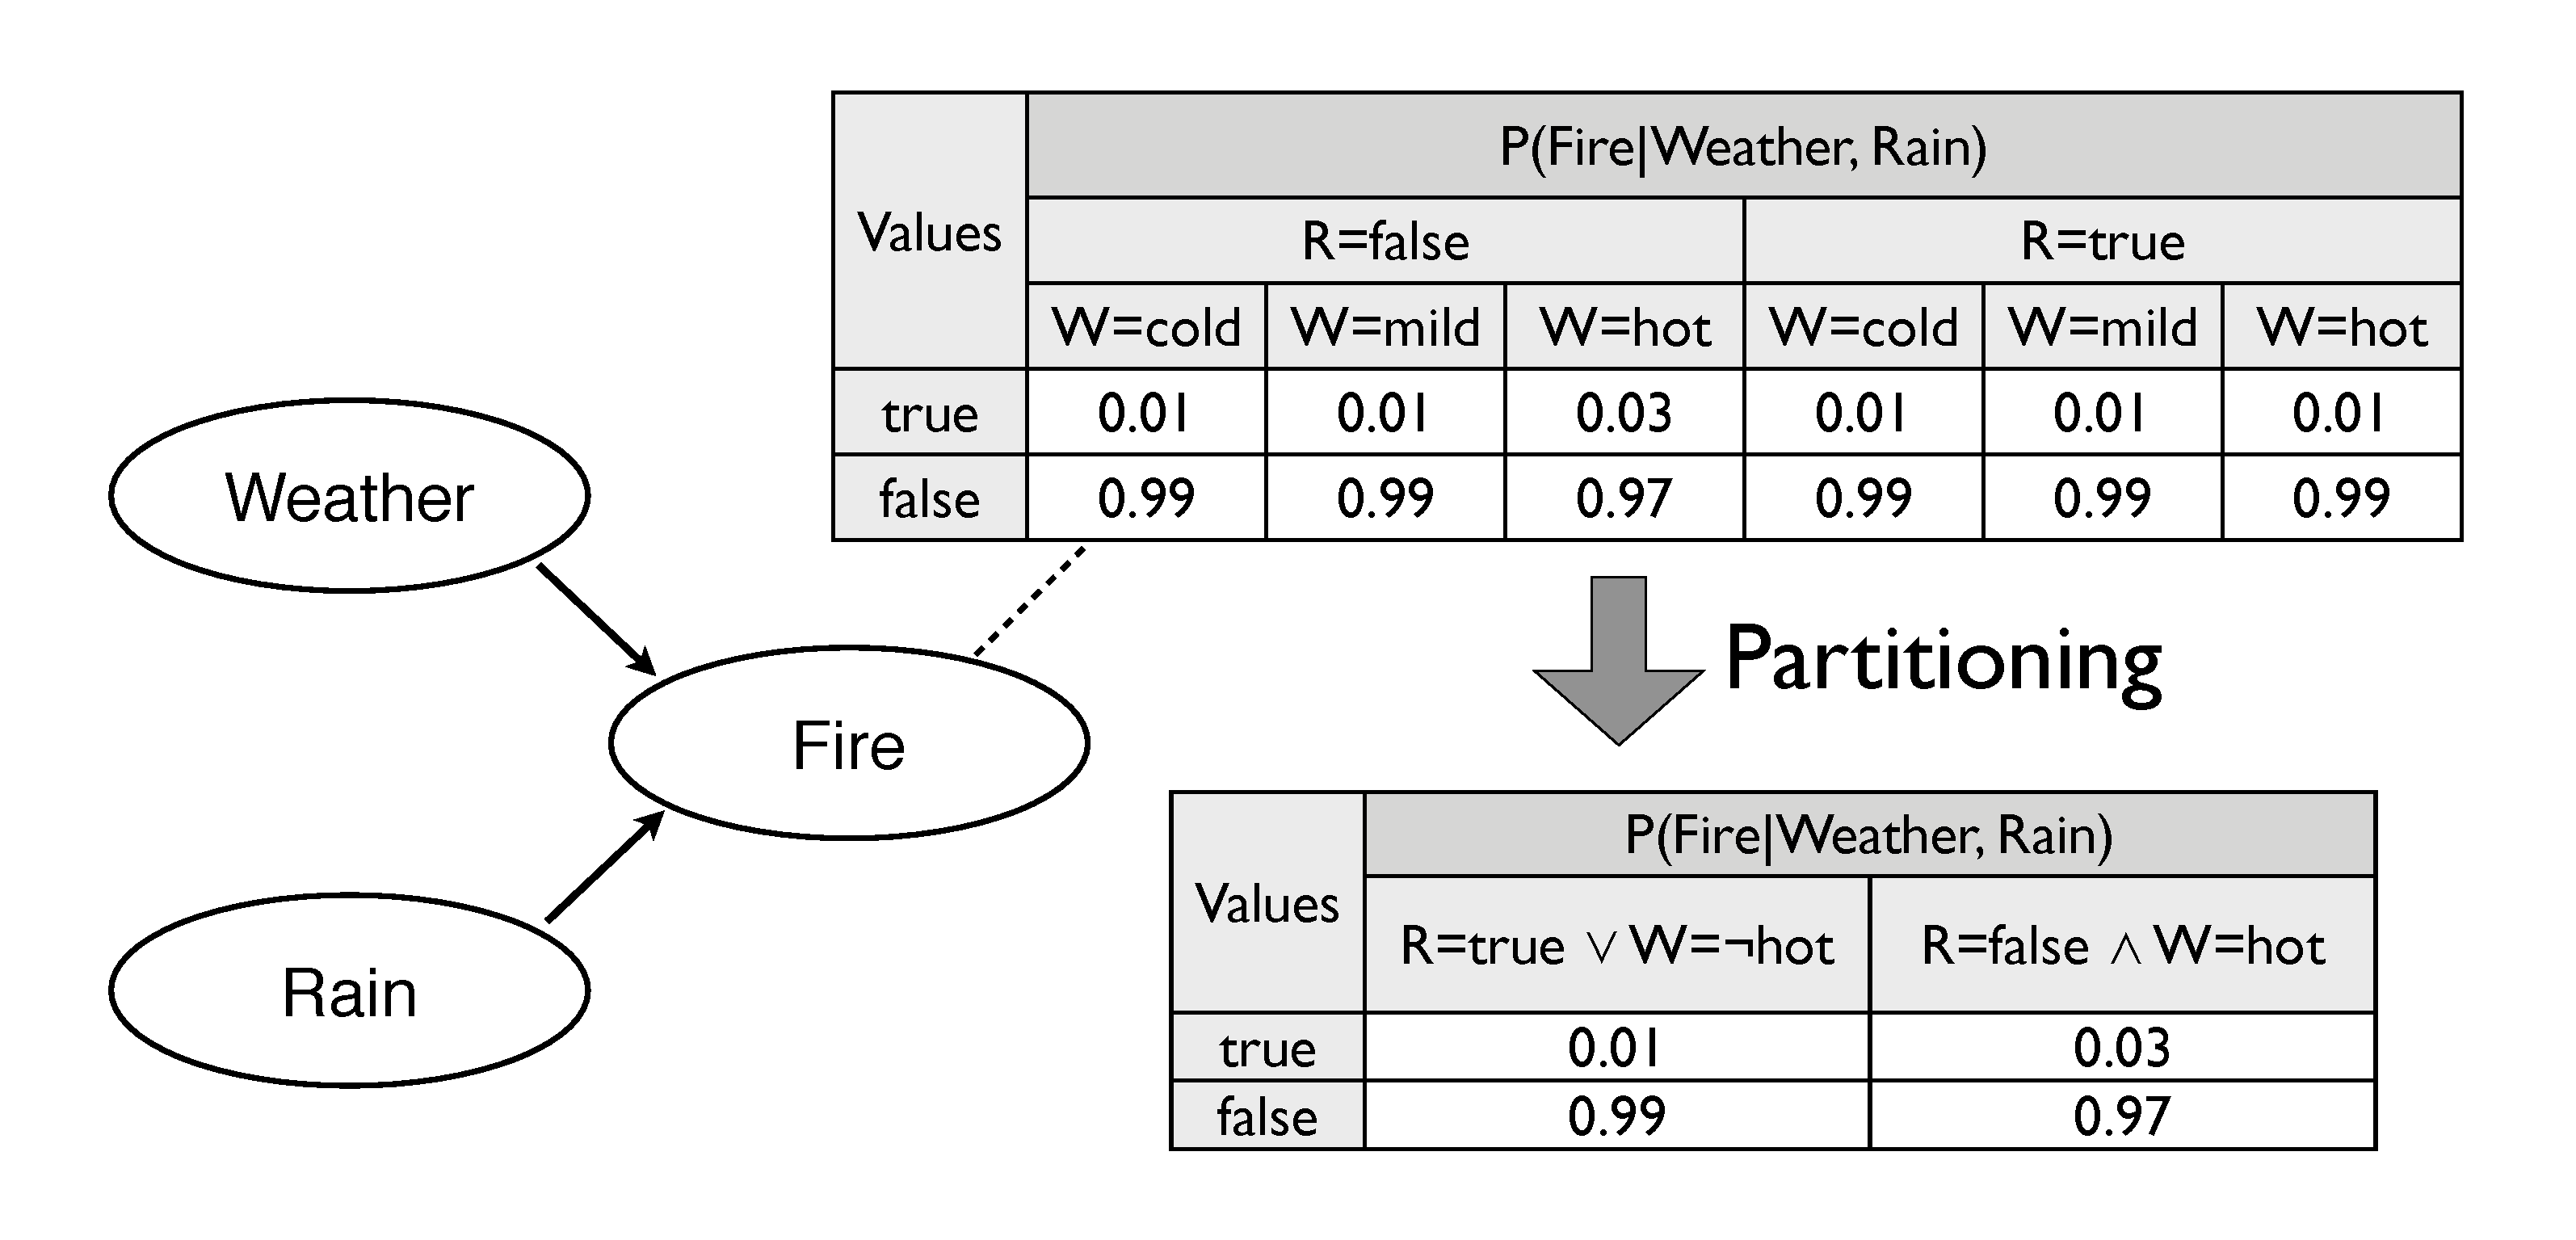
\includegraphics[scale=0.25]{imgs/partitioning.pdf}
\caption{Partitioning for the conditional probability distribution $P(\mathit{Fire} \, | \mathit{Weather}, \mathit{Rain})$.}
\label{fig:partitioning}
\end{figure}

Partitions must both exhaustive (each combination of values for the parent variables must belong to one partition) and mutually exclusive (a combination of values can only belong to one partition).  As we can observe from the example, partitions can often be concisely expressed via logical conditions on the variable values.  A given assignment of values will then be grouped in a partition if it satisfies the condition associated with it.

\subsubsection*{Quantification}

May domains present a rich relational structure of objects or abstract entities \citep{Otterlo2006,Getoor+al:SRL07}. Situated dialogue domains such as human-robot interaction belong in particular to this category.  These domains are often difficult to directly encode by a fixed set of random variables, as the number of entities and relations may vary over time.  Examples of such relational structure include: 
\begin{itemize}
\item Collections of physical objects in a visual scene, each described by specific features (colour, shape) and relations with other objects (e.g. spatial relations),
\item Indoor environments topologically structured in rooms and spaces in which to navigate. 
\item Stacks of tasks to complete by the agent, each task being possibly connected to other tasks via precedence or inclusion relationships.
\end{itemize}

First-order logic provides an excellent basis for representing and manipulating such relational structures, as it offers a rich language for (1) referring to objects connected with one another through functions and relations and (2) describing their properties in a concise way through the use of universal and existential quantifiers.\footnote{We shall not cover in this thesis the mathematical foundations of first-order logic, but the interested reader is invited to refer to e.g. \cite{gamut1991logic} for a formal overview of the logical concepts mentioned throughout this thesis.}

Graphical models can represent such relational domains by instantiating one random variable for every possible grounding of the functions and predicates for the domain.\footnote{Such operation is equivalent to \textit{propositionalisation} in the terminology of first-order logic.}  A domain with two objects $o_1$ and $o_2$ and a relation $\mathit{leftOf}(x,y)$ will for instance generate the four groundings $\mathit{leftOf}(o_1,o_2)$, $\mathit{leftOf}(o_2,o_1)$ $\mathit{leftOf}(o_1,o_1)$ and $\mathit{leftOf}(o_2,o_2)$. However, the definition of probability and utility distributions that can handle the relational semantics of such representation is not straightforward.  Many properties or constraints are indeed independent of the particular object being considered, such as $\forall x, \neg \mathit{leftOf}(x,x)$ and $\forall x, y, z, \mathit{leftOf}(x,y) \land \mathit{leftOf}(y,z) \Rightarrow \mathit{leftOf}(x,z)$. Classical probabilistic models offer unfortunately no direct support for quantifiers, as their expressive power is intrinsically limited to propositional logic. 
 
The unification of first-order logic and probability theory has spanned a new research area called \textit{statistical relational learning} \citep{getoor:srlbook07}. Many of the methods developed in this field operate by defining a logic-based description language on top of classical probabilistic models that allow for some form of quantification. This description language is then used as a template to generate a classical probabilistic model given a set of constants. The introduction of quantifiers provide another abstraction mechanism to reduce the complexity of a given probabilistic models by describing constraints or relations that hold for all possible groundings of a given formula and can therefore apply to a large set of random variables. 

\section{Formalisation}
\label{sec:formalisation}

We now outline a generic description framework for expressing the types of internal structure we have just detailed.  This description framework is based on the use of rules to structure conditional probability distributions and utility distributions.  The framework has originally been presented in \cite{rulebasedmodels-sigdial2012,lison-semdial2012}.  

The key idea is to represent distributions with the help of \textit{if ... then ... else} control blocks, based on the following skeleton:
\begin{equation*}
\begin{aligned}
& \textbf{if} \ \ (\text{condition 1 holds}) \ \ \textbf{then} \\ 
& \;\;\;\;\; \text{Distribution 1 over possible effects} \\
& \textbf{else if} \ \ (\text{condition 2 holds}) \ \ \textbf{then} \\ 
& \;\;\;\;\; \text{Distribution 2 over possible effects} \\
& ... \\
& \textbf{else} \\
& \;\;\;\;\; \text{Distribution } n \text{ over possible effects} \\ 
\end{aligned}
\label{eq:probrule}
\end{equation*}

Each \textit{if...then} case inside the block specifies both a \textit{condition} on particular state variables, and a distribution over possible \textit{effects}.   The \textit{if ... then ... else} structure is read in sequential order (as in most programming languages) until a satisfied condition is found, in which case the probabilistic effects associated with it are enacted.

We first present how rules can express conditional probability distributions in terms of structured (and parametrised) mappings between input and output variables.  We then show how to  generalise the formalism to utility distributions and extend it with quantification mechanisms.

\subsection{Basic definition}

Probabilistic rules take the form of \textit{if ... then ... else} control structures and map a list of conditions on input variables to probabilistic effects on output variables. More formally, a rule is expressed as an ordered list $\langle br_1, ... br_n\rangle$, where each branch $br_i$ is a pair $(c_i, P(E_i))$ where $c_i$ is a condition and $P(E_i)$ an associated distribution over possible effects.  The distribution $P(E_i)$ is a categorical distribution with possible effects $Val(E_i) = \{e_i^1,... e_i^{m_i}\}$, where $m_i$ is the number of alternative effects in $P(E_i)$.  Each effect $e_i^j \in Val(E_i)$ has a particular probability denoted $p_i^j$.  The probabilities $p_i^{1...m_i}$ must satisfy the usual probability axioms $p_i^j \geq 0 \ \forall i,j$ and $\sum_{j = 1}^m p_i^j = 1 \ \forall i$. 

Given these elements, a basic probabilistic rule reads as such:
\begin{equation}
\begin{aligned}
& \textbf{if} \ \ (c_{1}) \ \ \textbf{then} \\ 
& \;\;\;\;\; \begin{cases}
P(E_1\!=\!e_1^1) = p_1^1 \\
 ... \\
P(E_1\!=\!e_1^{m_1}) = p_1^{m_1} 
\end{cases} \\[3mm]
& \textbf{else if} \ \ (c_{2}) \ \ \textbf{then} \\ 
& \;\;\;\;\; \begin{cases}
P(E_2\!=\!e_2^1) = p_2^1, \\
 ... \\
P(E_2\!=\!e_2^{m_2}) = p_2^{m_2}
\end{cases} \\ 
& ...  \\
& \textbf{else} \\
& \;\;\;\;\; \begin{cases}
P(E_n\!=\!e_n^1) = p_n^1, \\
... \\
P(E_n\!=\!e_n^{m_n}) = p_n^{m_n}
\end{cases}
\end{aligned}
\label{eq:probrule}
\end{equation}

 In the rest of this thesis, we will often write $P(e_i^j)$ as a notational convenience for $P(E_i = e_i^j)$. 

%The three following sections describe how the conditions $c_i$, effects $e_i^j$ and associated effect probabilities $p_i^j$ are respectively defined. 

\subsubsection*{Conditions}

The conditions $c_i$ are expressed as formulae grounded in a subset of the state variables. This subset of state variables are the \textit{input variables} of the rule. Conditions can be arbitrarily complex logical formulae connected by conjunction, disjunction and negation, and can also include free variables. The examples of partition  $(\mathit{Rain}\!=\mathit{true} \lor \mathit{Weather}\!\neq\mathit{hot})$ and $(\mathit{Rain}\!=\mathit{false} \land \mathit{Weather}\!=\mathit{hot})$ in Figure \ref{fig:partitioning} are instances of valid conditions on the two input variables $Rain$ and $\mathit{Weather}$. 

Given that a rule is defined through a \textit{if ... then ... else} control structure, the partitioning is guaranteed by construction to be exhaustive and mutually exclusive (only one effect will be enacted for a given assignment of input values).  When provided with an assignment of values on the input variables, the conditions are tested in sequential order until one is satisfied. When no terminating \textbf{else} statement is explicitly put at the end of a rule, the framework inserts a final empty (i.e. always satisfied) condition associated with a void effect to ensure that the partitioning is exhaustive. 

The conditions on the input variables effectively provides a compact partitioning of the state space to mitigate the dimensionality curse.  Without this partitioning in alternative conditions, a rule ranging over $v$ input variables each of size $w$ would need to enumerate $v^w$ possible assignments.  Partitioning this space with conditions reduces this number to $n$ mutually exclusive partitions, where $n$ is usually small. 


\subsubsection*{Effects}

Associated to each condition $c_i$ stands a list of alternative, mutually exclusive effects $e_i^{1...m_i}$. Each effect $e_i^j$ defines a specific assignment of values for another subset of the state variables.  An effect is defined as a conjunction of (variable,value) pairs $X_1\!=\!x_1 \land X_2\!=\!x_2 \land ... X_k\!=\!x_k$ where $X_1,... X_k$ denote particular random variables in the dialogue state and $x_1,...x_k$ corresponding values for these variables.   The variables $X_1,...,X_k$ are the \textit{output variables} of the rules. In the partitioning example from Figure \ref{fig:partitioning}, the output variable is unique and corresponds to $Fire$. We shall however encounter some examples of rules with more than one output variable. It is also worth nothing that the sets of input and output variables can overlap.

Effects can be void -- that is, represent an empty assignment.  In such case, the effect does not lead to any change in the model distribution for the state variables. 

\subsubsection*{Probabilities}

Each effect $e_i^j$ is assigned with a probability $p_i^j = P(E_i = e_i^j)$.  These probabilities can be either 
fixed by hand or correspond to parameters to estimate from data. In the latter case, we adopt a Bayesian learning approach (cf. Section \ref{sec:learning}) and assume the probabilities $e_i^{1...m_i}$ to be drawn from the conjugate prior of categorical distributions: Dirichlet distributions. Chapters \ref{chap:wozlearning} and \ref{chap:rllearning} detail how Dirichlet distributions can be exploited to estimate probability parameters. 

It often happens that only the distribution $P(E_i)$ only includes one single effect with probability 1.  In such case, the rule is equivalent to a deterministic distribution. 

\subsubsection*{Example}

Rule $r_1$ illustrates a simple example of probabilistic rule:
\begin{align*}
r_1: \ \ \ \ \ & \textbf{if} \ (\mathit{Rain}\!=\!\mathit{false} \land \mathit{Weather}\!=\!\mathit{hot}) \ \textbf{then} \\
& \;\;\;\;\;  \begin{cases}
 P(\mathit{Fire}\!=\!\mathit{true}) = 0.03 \\ 
P(\mathit{Fire}\!=\!\mathit{false}) = 0.97
\end{cases} \\ 
& \textbf{else} \\
& \;\;\;\;\; \begin{cases}
P(\mathit{Fire}\!=\!\mathit{true}) = 0.01 \\
P(\mathit{Fire}\!=\!\mathit{false}) = 0.99
\end{cases} 
\end{align*}

Rule $r_1$ has two input variables: $\mathit{Rain}$ and $\mathit{Weather}$ as well as one output variable $\mathit{Fire}$. The rule specifies that the probability of a fire is 0.03 in case of no rain and a hot weather and 0.01 in all other cases.  The reliance on high-level conditions enables the conditional probability distribution to be specified with only four probabilities in comparison to 12 for the original conditional probability distribution shown in Figure \ref{fig:partitioning}. 

%Here is a first example of probabilistic rule pertaining to the user action model: 
%\begin{align*}
%\textbf{Rule 1}: \ \ & \textbf{if} \ (\exists X: a_m=\mathit{Confirm(X)} \land i_u = \mathit{X})  \ \textbf{then} \\ 
%& \;\;\;\;\; \{[P(a_u' = \mathit{Confirm}) = 0.9]\} \\
%& \textbf{else if} \ (\exists X: a_m=\mathit{Confirm(X)} \land i_u \neq \mathit{X})  \ \textbf{then} \\ 
%& \;\;\;\;\; \{[P(a_u' = \mathit{Disconfirm}) = 0.95]\}
%\end{align*}
%The rule specifies that, if the system requests the user to confirm that his intention is $X$ and his actual intention is indeed $X$, the user is expected to utter a $\mathit{Confirm}$ action with probability 0.9.  Otherwise, the rule produces a void effect -- i.e. it leaves the distribution $P(a_u')$ unchanged. If the intention is different, the user will utter a $\mathit{Disconfirm}$ action with  probability 0.95.   

\subsection{Utility distributions}

The rule-based formalism we have outlined can also be used to described utility distributions using only minor notational changes. Utility rules essentially retain the same form as probabilistic rules, with one notable exception, namely that the probabilistic effects are replaced by utility distributions over particular assignments of decision variables. 

Formally, a utility rule is an ordered list $\langle br_1, ... br_n\rangle$, where each branch $br_i$ is a pair $(c_i, U(D_i))$ where $c_i$ is a condition and $U(D_i)$ an associated utility distribution over possible assignments of decision variables. The utility distribution $U(D_i)$ specifies a set of possible decisions  $Val(D_i) = \{d_i^1,... d_i^{m_i}\}$.  Each decision $d_i^j \in Val(D_i)$ has a particular utility value denoted $u_i^j$.  Utility rules can be expressed in the following manner:
\begin{equation}
\begin{aligned}
& \textbf{if} \ \ (c_{1}) \ \ \textbf{then} \\ 
& \;\;\;\;\; \begin{cases}
U(D_1\!=\!d_1^1) = u_1^1 \\
 ... \\
U(D_1\!=\!d_1^{m_1}) = u_1^{m_1} 
\end{cases} \\
& ...  \\
& \textbf{else} \\
& \;\;\;\;\; \begin{cases}
U(D_n\!=\!d_n^1) = u_n^1, \\
... \\
U(D_n\!=\!d_n^{m_n}) = u_n^{m_n}
\end{cases}
\end{aligned}
\end{equation}

Informally, a utility rule stipulates the utility values associated with particular system decisions depending on conditions on the state variables.  As for probabilistic rules, the conditions $c_i$ are defined as arbitrary logical formulae on a subset of state variables.  The decisions $d_i^j$ are assignments $X_1\!=\!x_1 \land X_2\!=\!x_2 \land ... \land X_n\!=\!x_n$ where the variables $X_1,..X_n$ are decision variables and $x_1,...x_n$ possible values for these variables. The utility values $u_i^j$ are real numbers. 

Although most utility rules only include one single decision variable, the possibility to integrate multiple decision variables is helpful in domains where the system can execute multiple actions in parallel. Such situations frequently arise in human-robot interaction and multi-modal applications, as the system can communicate through both verbal and non-verbal channels and is often able to perform physical actions in addition to communicative acts. 
 
\subsubsection*{Example}

Rule $r_2$ provides a simple example of utility rule:

\begin{align*}
r_2: \ \ & \textbf{if} \ (\mathit{Fire}\!=\!\mathit{true}) \ \textbf{then} \\
& \;\;\;\;\;  \begin{cases}
U(\mathit{Tanker}\!=\!\mathit{dropWater}) = 5 \\
U(\mathit{Tanker}\!=\!\mathit{wait}) = -5
\end{cases} \\
& \textbf{else} \\
& \;\;\;\;\; \begin{cases}
U (\mathit{Tanker}\!=\!\mathit{dropwater}) = -1 \\
U(\mathit{Tanker}\!=\!\mathit{wait}) = 0
\end{cases}
\end{align*}

Rule $r_2$ stipulates that the respective utility of the two action values for the decision variable $\mathit{Tanker}$ depending on a condition on the state variable $\mathit{Fire}$. 

\subsection{Quantification}
\label{sec:quantification}

Quantifiers are an important mechanism to abstract over particular relational aspects of the domain structure.  Variables can be included in the specification of both the conditions and effects of a given rule, and are universally quantified on top of the rule.\footnote{These variables are variables in the sense of first-order logic, and is not to be confused with the random variables of the probabilistic model.}  A rule containing the free variables $x_1,x_2,...x_k$ in its conditions and/or effects is therefore written as:
\begin{equation}
\begin{aligned}
\forall \mathbf{x} = x_1, x_2,...x_k: \\
& \textbf{if} \ \ (c_{1}(\mathbf{x})) \ \ \textbf{then} \\ 
& \;\;\;\;\; \begin{cases}
P(E_1\!=\!e_1^1(\mathbf{x})) = p_1^1 \\
 ... \\
P(E_1\!=\!e_1^{m_1}(\mathbf{x})) = p_1^{m_1} 
\end{cases} \\ 
& ...  \\
& \textbf{else} \\
& \;\;\;\;\; \begin{cases}
P(E_n\!=\!e_n^1(\mathbf{x})) = p_n^1, \\
... \\
P(E_n\!=\!e_n^{m_n}(\mathbf{x})) = p_n^{m_n}
\end{cases}
\end{aligned}
\label{eq:rulewithquant}
\end{equation}

The formalisation allows certain variables $x_1,...x_k$ in the conditions and effects to be \textit{underspecified}.  The mapping between conditions and effects specified by the rule is therefore instantiated for every possible assignment of the underspecified variables. The quantification mechanism introduced in \eqref{eq:rulewithquant} enables probabilistic rules to cover large portions of the state space in a highly compact manner, based on a reduced number of parameters. One of the key advantages of such representation is it allows for powerful forms of \textit{parameter sharing}, as the effect probabilities $p_i^j$ in the above rule are made independent of the various possible instantiations of the variables $x_1,...x_k$. Quantification can also be used for utility rules in the same manner. 

\subsubsection*{Example}

Rule $r_3$ is an example of rule that employs quantification on two variables denoted $o$ and $c$.\footnote{Note the absence of an explicit final \textit{else} branch, which is then by default associated with an empty effect.}
\begin{align*}
r_3: \ \ & \forall o, c: \\ 
& \textbf{if} \ (a_m\!=\!\mathit{WhatIsColour}(o) \land \mathit{colour}(o)\!=\!\mathit{c})  \ \textbf{then} \\ 
& \;\;\;\;\; \begin{cases} P(a_u'=\mathit{Assert}(\mathit{HasProperty}(o,\mathit{c}))) = 0.95 \end{cases}
\end{align*}

Rule $r_3$ is used to predict the next user dialogue act $a_u'$ after a system-initiated question such as ``What colour is the object'' depending on the colour of the object that is referred to. The rule assumes the presence in the dialogue state of a random variable $colour(o_i)$ for each object $o_i$ perceived by the system. The rule specifies that the user is likely (with probability 0.95) to utter a dialogue act such as ``the object is X'' at the next turn, where X is the actual colour of the object. Otherwise no prediction is made. If the dialogue state contains e.g. one object $o_1$ with $P(\mathit{colour}(o_1)=blue)=0.8$ and the last system action was $WhatIsColour(o_1)$, the probability of the user uttering ``the object is blue'' is therefore $0.76$.  It is worth observing in this example that the variables $o$ and $c$ are allowed to occur both inside the name of a random variable, as in $\mathit{colour}(o)$, and inside the value of a random variable, as in $\mathit{WhatIsColour(o)}$, $c$ and $\mathit{Assert}(\mathit{HasProperty}(o,\mathit{c}))$. 

\section{Rule instantiation}
\label{sec:ruleinstantiation}

The rules are instantiated at runtime in the dialogue state by creating a distinct chance node for every rule.  These rule nodes are essentially latent variables that serve as intermediaries between input and output variables.  Albeit the occurrence of these rules is never directly observed, they help structuring the relations between variables and enable the system designer to decompose complex probability and utility models into smaller parts.  

The dialogue state is in our approach represented as a Bayesian network of state variables, in line with other dialogue management approaches such as \cite{Thomson:2010:BUD:1772996.1773040,bui2010}. Rules are then applied upon this dialogue state.  Probabilistic rules are employed to create or update particular state variables, whereas utility rules define decision variables and their corresponding utility values. The instantiated rules are equivalent to a dynamic decision network (cf. previous chapter). 

We describe below the instantiation procedure for each type of rule. For simplicity's sake, we shall first limit our discussion to rules without quantifiers, and then show quantifiers can be accounted for in the instantiation process. 

\subsection{Probability rules}
\label{sec:probruleinstantiation}

Let $\mathcal{B}$ be the Bayesian network representing the current dialogue state, and $\mathcal{R}$ a set of rules to apply to this dialogue state.  For each rule $r \in \mathcal{R}$, a chance node is created.  This chance node represents a random variable on the possible effects of the rule.  The node is conditionally dependent on the input variables of the rule (i.e. the set of all variables that are mentioned in the rule conditions), and is also connected via outgoing edges to its output variables (i.e. the set of all variables that are mentioned in the rule effects). 

Figure \ref{fig:instantiationprob} illustrates this construction process on an artificial example.  The two rules $r_4$ and $r_5$ are applied on the state variables $A$, $B$, $C$ and $D$.  The application of the two rules results in an update of the variable $A$ and the creation of a new variable $E$. The random variable represented by the node $r_4$ has three possible values, reflecting the effects described in the rule: $Val(r_4) = \{ [A\!=\!a_1], [A\!=\!a_2], \{\cdot\}\}$.  Note that $\{\cdot\}$ denotes the empty effect.  Similarly, the random variable $r_5$ has four alternative effects: $Val(r_5) = \{[A\!=\!a_2 \land E\!=\!e_2], [A\!=\!a_2 \land E\!=\!e_1], [E=e_2], \{\cdot\}\}$. 

\begin{figure}[h]
\centering
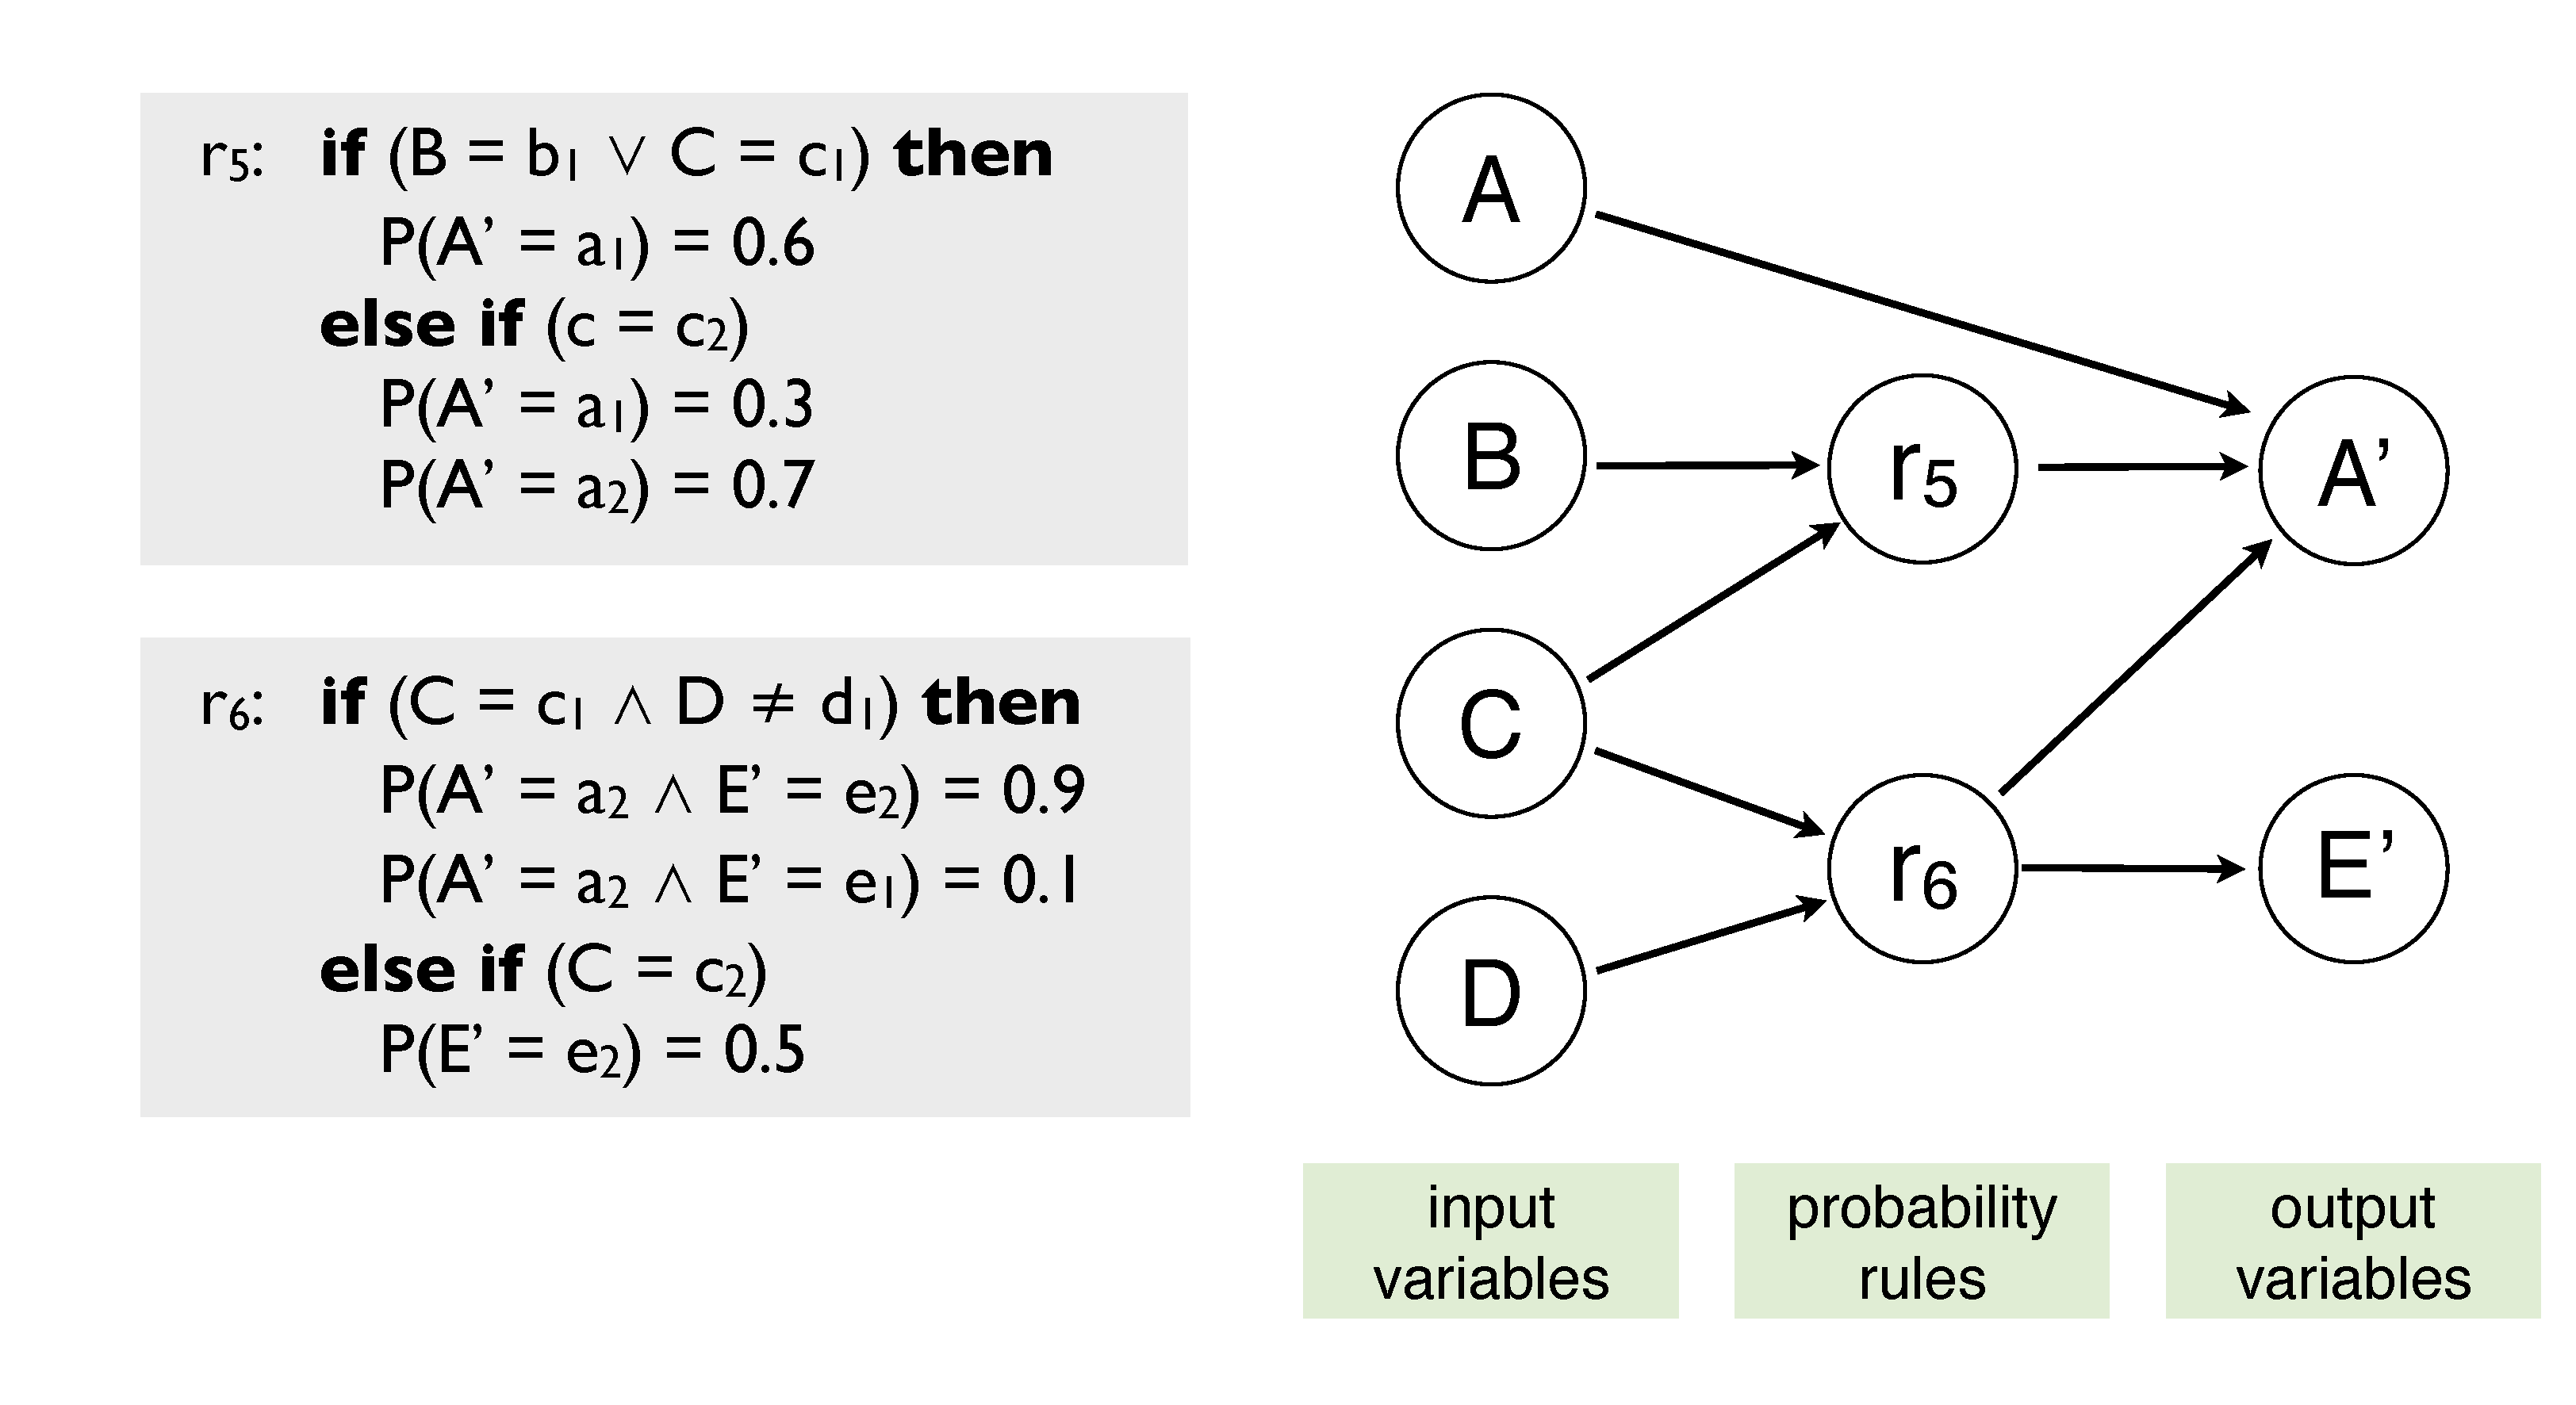
\includegraphics[scale=0.25]{imgs/ruleinstantiation.pdf}
\caption{Example of instantiation for the two probability rules $r_4$ and $r_5$. The remaining probability mass in the rule specifications is by default assigned to the empty effect. }
\label{fig:instantiationprob}
\end{figure}

We shall adopt the following terminology for the distributions created through the instantiation procedure: 
\begin{itemize}
\item The conditional probability distribution associated with rule nodes such as $r_4$ and $r_5$ given their inputs is a \textit{rule distribution}.
\item The conditional probability distribution associated with output variables such $A'$ and $E'$ given the rule nodes that affect it is a \textit{output distribution}.
\end{itemize}

\subsubsection*{Rule distributions}

The conditional probability distribution of a rule $r$ given its input variables $I_1,...I_n$ is defined as: 
\begin{align}
& P(r\!=\!e \, | \, I_1\!=\!i_1,... I_n\!=\!i_n) = P(E_i = e) \label{eq:ruledistrib}
 \\ 
& \; \; \; \; \; \; \; \; \text{ where } i = \min_i (c_i \text{ is satisfied with } I_1\!=\!i_1 \land ... I_n\!=\!i_n) \nonumber 
\end{align}
In other words, the rule conditions are checked in sequential order until one condition $c_i$ is satisfied for the given input.  The distribution for the rule is then simply determined as the effect distribution $P(E_i\!=\!e)$ associated with the satisfied condition $c_i$. 

As an example, the rule distribution $P(r_4 \, | \, B\!=\!b_1, C\!=\!c_1)$ for the node $r_4$ in Figure \ref{fig:instantiationprob} is defined as:
\begin{itemize}
\item $P(r_4 = \{A\!=\!a_1\} \, | \, B\!=\!b_1, C\!=\!c_1) = 0.6$
\item  $P(r_4 = \{\cdot\} \, | \, B\!=\!b_1, C\!=\!c_1) = 0.4$
\item $P(r_4 = \{A\!=\!a_2\} \, | \, B\!=\!b_1, C\!=\!c_1) = 0$
\end{itemize}
Similarly, the distribution $P(r_5 \, | \, C\!=\!c_1, D\!=\!d_1)$ is a deterministic distribution with the empty effect $\{\cdot\}$ assigned to a probability 1. 

\subsubsection*{Output distributions} 

An output variable $X'$ is conditionally dependent on all the rule nodes that refer to it in their effects.  In addition, output variables that result in the update of existing variables also include a conditional dependence on these existing variables. The output distribution is a direct reflection of the effects specified in the rules. The conditional probability distribution $P(X'|r_1\!=\!e_1,...r_n\!=\!e_n)$ for an output variable $X'$ with $n$ incoming rule nodes is defined in the following manner:
\begin{align}
&P(X'\!=\!x' \, | \, r_1\!=\!e_1,... r_n\!=\!e_n) = \begin{dcases}
\frac{\sum_{v \in {\mathbf{e}(X)}} \mathbf{1}(x' = v)} { |\mathbf{e}(X)| } & \text{if } \mathbf{e}(X)\!\neq\!\emptyset \\
\mathbf{1}(x' = \mathit{None}) & \text{otherwise}
\end{dcases}
\label{eq:outputdist1}
\end{align}
where the following notation is used: \begin{itemize}
\item $\mathbf{e}$ is the conjunction of all effects, i.e. $\mathbf{e} = e_1 \land ... e_n$.  Note that this conjunction can include several value assignments for a given variable.
\item $\mathbf{e}(X)$ denotes the (possibly empty) set of values specified for the variable $X$ in $\mathbf{e}$. 
\item $\mathbf{1}(p)$ is the indicator function for the Boolean $p$, with $\mathbf{1}(p)=1$ if $p$ is true and $0$ otherwise.
\end{itemize}

Equation \eqref{eq:outputdist1} stipulates that the distribution for $X'$ will follow the values assigned in the effect(s) provided that at least one effect specifies a value for it. If the effects include conflicting assignments, the distribution is spread uniformly over the alternative values. If all effects $e_1,...e_n$ are empty assignments, the value for $X'$ is set to a default $None$ value.

In case the variable $X'$ is an update of an existing variable $X$, the procedure remains essentially the same as for \eqref{eq:outputdist1}, except that the distribution for $X'$ will follow the one for the existing variable $X$ instead of being assigned a $\mathit{None}$ value in the case where all the effects specify empty assignments for the variable: 
\begin{align}
&P(X'\!=\!x' \, | \, r_1\!=\!e_1,... r_n\!=\!e_n, X\!=\!x) = \begin{dcases} 
\frac{\sum_{v \in {\mathbf{e}(X)}} \mathbf{1}(x' = v)} { |\mathbf{e}(X)| }  & \text{if } \mathbf{e}(X)\!\neq\!\emptyset \\
\mathbf{1}(x' = x) & \text{otherwise}
\end{dcases}\label{eq:outputdist2}
\end{align}

As an example, the output distribution $P(A' \, | \, r_4\!=\!\{\cdot\},r_5\!=\!\{A\!=\!a_2 \land E\!=\!e_2\}, A\!=\!a_3)$ for the variable $A'$ in Figure \ref{fig:instantiationprob} results in a deterministic distribution with a unique value $a_2$ with probability 1.  If the two rules generate conflicting assignments, the probability mass is divided equally over the alternative values -- for instance, the distribution $P(A' \, | \, r_4\!=\!\{A\!=\!a_1\},r_5\!=\!\{A\!=\!a_2 \land E\!=\!e_2\}, A\!=\!a_3)$ is a uniform distribution with two values: $a_1$ and $a_2$, each with probability 0.5. Finally, if all effects are empty, the output distribution is a simple copy of the distribution for the existing variable: $P(A' \, | \, r_4\!=\!\{\cdot\},r_5\!=\!\{\cdot\}, A\!=\!a_3)$ has a unique value $a_3$ with probability 1. 

It is worth noting that such output distribution is entirely parameter-free, as it is directly derived from the specified effects in the rule node.  The ordering of the rule parents in the distribution is arbitrary. The resulting distribution bears resemblance to the probabilistic Independence of Causal Influence (pICI) described by \cite{diez06}. 


\subsubsection*{Instantiation algorithm} 
\label{sec:utilruleinstantiation}

The procedure for instantiating a rule in a given state is detailed in Algorithm \ref{algo:instantiateProbRule}.  The first steps are to extract the input variables for the rule in the Bayesian network (line 1), create a node corresponding to the rule (line 2) and include its conditional dependences (line 3).  The algorithm then checks whether at least one effect in $R$ is non-empty given its conditional dependences (lines 4).  If all effects are empty, the rule node is irrelevant and can be directly pruned (line 5). Otherwise, the output variables are extracted (line 7), and output nodes that do not already exist in the network are created (line 10-11). The final step is to establish  dependency edges between the rule node and these output variables (line 13).

\begin{algorithm}[h!]
\caption{: \textsc{InstantiateProbRule} ($\mathcal{B}, r$)}
\begin{algorithmic}[1] \vspace{1mm}
\REQUIRE $\mathcal{B}$: Bayesian network for the current state
\REQUIRE $r$: Probability rule to instantiate in network  \vspace{1mm}
\STATE $\mathcal{I}_{r} \leftarrow$ input variables for rule $r$
\STATE Create chance node $R$ with the rule distribution in Eq. \eqref{eq:ruledistrib}
\STATE Add node $R$ and dependency edges $\mathcal{I}_{r} \rightarrow R$ to $\mathcal{B}$ 
\IF {$Val(R) = \{\cdot\}$}
\STATE Prune $R$ from $\mathcal{B}$
\ELSE
\STATE $\mathcal{O}_{r} \leftarrow$ output variables mentioned in the effects of $R$
\FORALL {output variable $O \in \mathcal{O}_r$}
\IF {$O'$ not already in $\mathcal{B}$}
\STATE Create chance node $O'$ with the output distribution in Eq. \eqref{eq:outputdist1}
\STATE Add node $O'$ and (in case $O$ exists) dependency edge $O \rightarrow O'$ to $\mathcal{B}$
\ENDIF
\STATE Add dependency edge $R \rightarrow O'$ to $\mathcal{B}$ 
\ENDFOR
\ENDIF
\end{algorithmic}
\label{algo:instantiateProbRule}
\end{algorithm}

\subsection{Utility rules}

Utility rules are instantiated in the Bayesian network following a similar procedure, with two notable differences compared to probability rules: \begin{itemize}
\item As utility rules define utility distributions, their instantiation correspond to utility nodes instead of chance nodes.
\item Instead of output variables, the rules are associated with decision variables.  The association direction is inverted, as the decision node must be input to the utility node.
\end{itemize} 

Figure \ref{fig:instantitionutil} illustrates the instantiation of two utility rules $r_6$ and $r_7$. 

\begin{figure}[h]
\centering
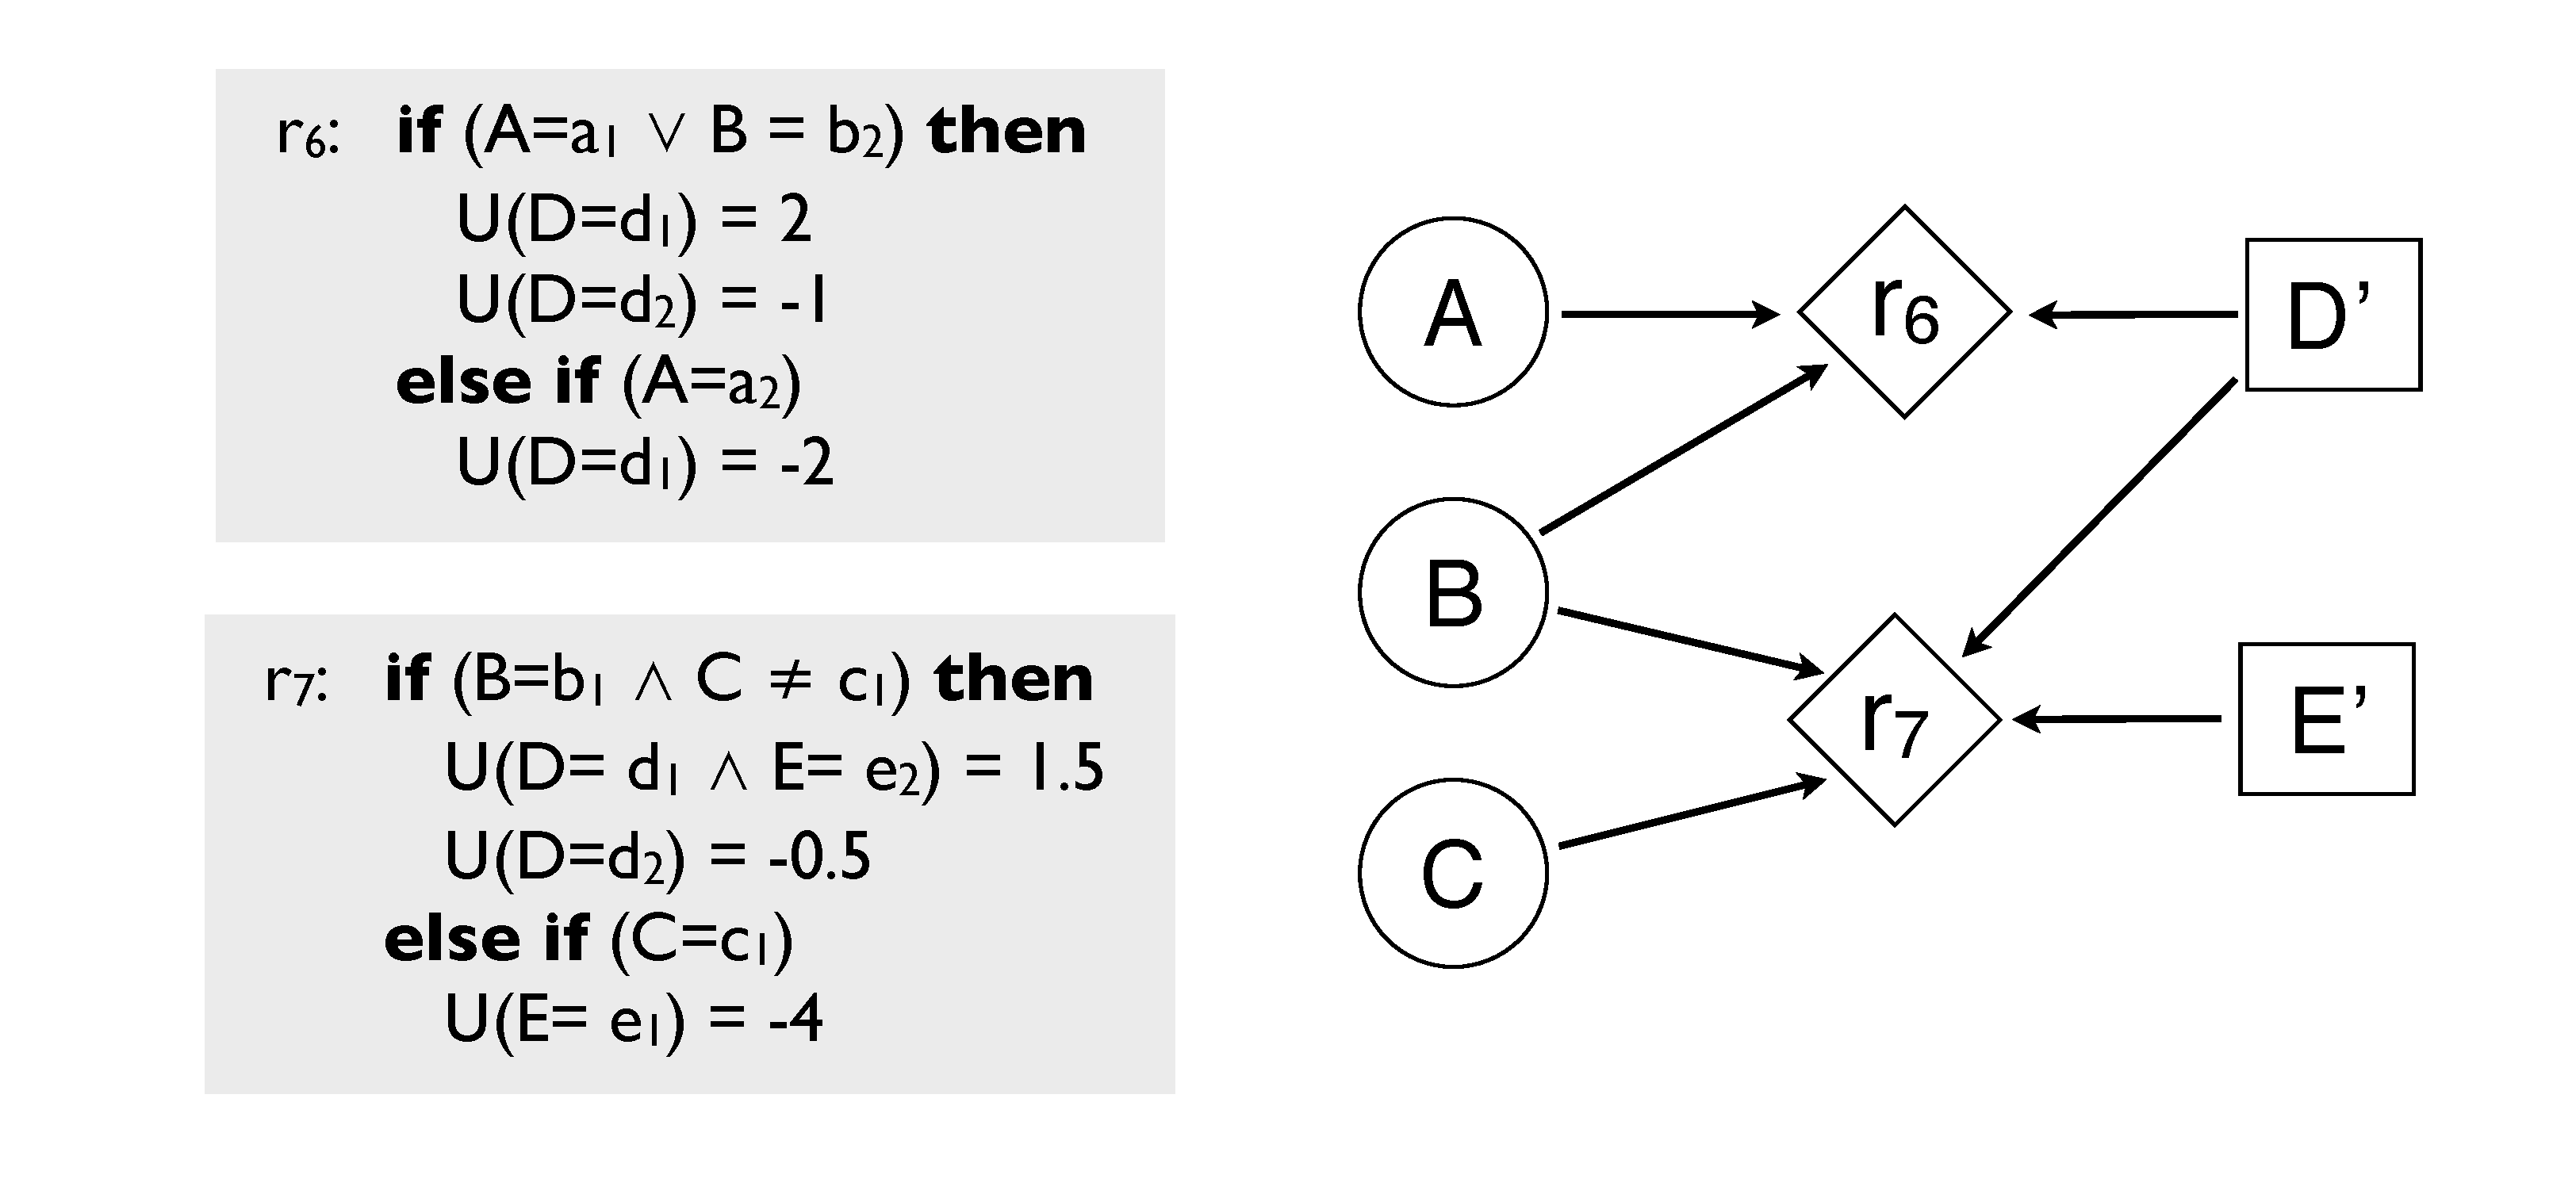
\includegraphics[scale=0.25]{imgs/ruleinstantiation2.pdf}
\caption{Example of instantiation for the two utility rules $r_6$ and $r_7$.}
\label{fig:instantitionutil}
\end{figure}


The utility distribution associated with each rule is a direct translation of the rule structured if...then...else mapping.  Formally, the utility distribution generated by a rule $r$ with input variables $I_1,...I_n$ and decision variables $A_1,...A_m$ is defined as:
\begin{align}
& U_r(I_1\!=\!i_1,... I_n\!=\!i_n, A_1\!=\!a_1,... A_m\!=\!a_m) = \nonumber \\ 
& \; \; \; \; \; \; \; \; U(D_i = \{A_1\!=\!a_1 \land... A_m\!=\!a_m\}) \label{eq:utildistrib}\\
&  \; \; \; \; \; \; \; \; \text{ where } i = \min_i (c_i \text{ is satisfied with } I_1\!=\!i_1 \land ... I_n\!=\!i_n) \nonumber
\end{align}

If no utility is explicitly specified for $\{A_1\!=\!a_1 \land... A_m\!=\!a_m\}$, the default value is zero. 

As is conventionally assumed in decision models, the total utility for a given assignment of decision variables is defined as the sum of all utilities.  The total utility for the actions $D'\!=\!d_1 \land E'\!=\!e_1$ in the case where $A\!=\!a_1$, $B=\!=\!b_1$ and $C\!=\!c_1$ is for instance equal to $2 - 4 = -2$. 


\subsubsection*{Instantiation algorithm} 

The procedure for instantiating a utility rule is similar in most respects to the one already outlined for probability rules. Algorithm \ref{algo:instantiateUtilRule} details the procedure, starting from the extraction of the input variables, the creation of the rule node, and the inclusion of conditional dependences (line 1-3). The algorithm then checks if at least the utility distribution stipulates a non-zero utility for at least one action (line 4).  If not, the node is irrelevant and can be pruned (line 5).  The decision variables associated with the rule are extracted (line 7), and a corresponding decision node is created if it does not already exists (line 10). Finally, the possible values specified for the decision variable are integrated to the node (line 12), and a dependency edge is established between the decision and utility nodes (line 13). 

\begin{algorithm}[h!]
\caption{: \textsc{InstantiateUtilRule} ($\mathcal{B}, r$)}
\begin{algorithmic}[1] \vspace{1mm}
\REQUIRE $\mathcal{B}$: Bayesian network for the current state
\REQUIRE $r$: Utility rule to instantiate in network  \vspace{1mm}
\STATE $\mathcal{I}_{r} \leftarrow $ input variables for rule $r$
\STATE Create utility node $R$ with the utility distribution in Eq. \eqref{eq:utildistrib}
\STATE Add node $R$ and dependency edges $\mathcal{I}_{r} \rightarrow R$ to $\mathcal{B}$ 
\IF {utility distribution is empty for all inputs}
\STATE Prune $R$ from $\mathcal{B}$
\ELSE
\STATE $\mathcal{D}_{r} \leftarrow$ decision variables defined for $R$
\FORALL {decision variable $D \in \mathcal{D}_r$}
\IF {$D'$ not already in $\mathcal{B}$}
\STATE Create decision node $D'$ and add it to $\mathcal{B}$
\ENDIF
\STATE Add in $Val(D')$ all possible values specified for it in the effects of $R$
\STATE Add dependency edge $D' \rightarrow R$ to $\mathcal{B}$ 
\ENDFOR
\ENDIF
\end{algorithmic}
\label{algo:instantiateUtilRule}
\end{algorithm}

\subsection{Application of quantifiers}

We saw in Section \ref{sec:quantification} that the conditions and effects of a rule could include universally quantified variables, but have not yet discussed how such underspecified rules could be practically instantiated in the Bayesian network. The general instantiation principle remains unchanged: to each rule corresponds a distinct rule node responsible for the mapping between input and output variables (or decision variables for utility rules). However, the instantiation procedure must be extended in a number of ways to accommodate the presence of underspecified variables. First, the extraction of input variables (line 1 in Algorithms \ref{algo:instantiateProbRule} and \ref{algo:instantiateUtilRule}) is not as straightforward, since the random variable names may be underspecified.  Second, the internal probability and utility distributions created by the rule must be adapted to account for the presence of quantifiers. 

\subsubsection*{Extraction of input variables}

Rules including quantifiers may underspecify the names of random variables.  Rule $r_3$ includes for instance a reference to an underspecified random variable $\textit{colour}(o)$, where $o$ is universally quantified.  In order to instantiate the rule, the system must therefore find all random variables included in the model that match the underspecified description. If rule $r_3$ is instantiated on a state containing two objects $o_1$ and $o_2$, the input variables will therefore be $\mathit{colour}(o_1)$ and $\mathit{colour}(o_2)$. 

Algorithm \ref{algo:getinputvariables} details how this search for matching input variables can proceed. The algorithms starts by extracting the initial input variables for the rule (that may include underspecified variables), and loops on each underspecified variable to find possible groundings in the Bayesian network.  The final result is defined as the combination of the fully specified variables for the rule and the possible groundings for the underspecified variables. 

\begin{algorithm}[h!]
\caption{: \textsc{GetInputVariables} ($\mathcal{B}, r$)}
\begin{algorithmic}[1] \vspace{1mm}
\REQUIRE $\mathcal{B}$: Bayesian network for the current state
\REQUIRE $r$: Probability or utility rule  \vspace{1mm}
\STATE $\mathcal{I}_{r} \leftarrow $ Initial (possibly underspecified) input variables for rule $r$
\STATE $\mathcal{U}_{r} \leftarrow $ Subset of variables in $\mathcal{I}_{r}$ that are underspecified
\STATE $\mathcal{G}_{r} \leftarrow$ possible groundings for underspecified variables $\mathcal{U}_{r}$, initialised to $[ \cdot ]$
\FOR {underspecified variable $u \in \mathcal{U}_{r}$}
\FOR {random variable $X$ in $\mathcal{B}$}
\IF {$X$ matches $u$}
\STATE $\mathcal{G}_{r} \leftarrow \mathcal{G}_{r} \cup [X]$
\ENDIF
\ENDFOR
\ENDFOR
\RETURN $(\mathcal{I}_{r} \ \backslash \ \mathcal{U}_{r}) \ \cup \  \mathcal{G}_{r}$
\end{algorithmic}
\label{algo:getinputvariables}
\end{algorithm}

Note that use of quantification on the random variable names may lead to a rapid increase in the number of parent variables for the rule node, and must be used with parsimony to ensure the inference problem remains tractable.  

\subsubsection*{Rule distribution with quantifiers}

We have seen in Section \ref{sec:probruleinstantiation} that probability rules were instantiated as a distinct node associated with a rule distribution, and that this node was connected to a set of output variables, each of which defined by an output distribution.  

 We can extend rule distributions defined in Equation \eqref{eq:ruledistrib} to incorporate quantified variables.  Let us assume a rule $r$ with input variables $I_1,...I_n$ and quantified over $\mathbf{x}$.  Given a particular assignment for the input variables $I_1,...I_n$, each rule condition $c_i$ is checked to find all possible groundings of $\mathbf{x}$  that makes $c_i$ satisfied.  Note that the number of groundings can be zero if the condition can never be satisfied. The result of this operation is a set of groundings $G= \mathbf{g}_1,...\mathbf{g}_{|G|}$ where each grounding must satisfy least one condition given the input assignment.\footnote{This method of handling quantifiers by extracting all possible groundings is an instance of \textit{ground inference} \citep{getoor:srlbook07}. The possible groundings for a given input must be in this setting restricted to a finite set. In order to retain tractability, the maximum number of groundings is also capped by a threshold.} Algorithm \ref{algo:getgroundings} shows how groundings can be extracted given a rule and a particular input assignment for it. $\phi[a/b]$ denotes (as in mathematical logic) the expression $\phi$ where all instances of the variable $a$ are substituted by $b$.
 
 %Groundings that satisfy a condition leading to an empty effect can be discarded. 
 
\begin{algorithm}[h!]
\caption{: \textsc{GetGroundings} ($r, \{I_1\!=\!i_1 \land ... I_n\!=\!i_n\}$)}
\begin{algorithmic}[1] \vspace{1mm}
\REQUIRE $r$: Probability or utility rule 
\REQUIRE $\{I_1\!=\!i_1 \land ... I_n\!=\!i_n\}$ assignment for the parent variables of the rule  \vspace{1mm}
\STATE $G \leftarrow \emptyset$
\FOR {$i = 1 \to n$}
\STATE Let $\mathbf{x}_i$ be the quantified variables in condition $c_i$
\STATE $G_i \leftarrow \{\text{grounding } \mathbf{g}_k \text{ of } \mathbf{x}_i: \ I_1\!=\!i_1 \land ... I_n\!=\!i_n \vdash c_i [\mathbf{g}_k / \mathbf{x}_i ]\}$
\STATE $G \leftarrow G \cup G_i$
\ENDFOR
\RETURN $G$
\end{algorithmic}
\label{algo:getgroundings}
\end{algorithm}
 
 Each grounding $\mathbf{g}_k \in G$ gives rise to a particular effect distribution, and the total effect for the rule is the conjunction of effects $[e_1 \land ... e_{|G|}]$ for all possible groundings.  The probability of each conjunction is defined as the product of probabilities for the grounding-specific effects:
\begin{align}
& P(r\!=\![e_1 \land ... e_{|G|}] \, | \, I_1\!=\!i_1,... I_n\!=\!i_n) = \prod_{k=1}^{|G|} P(E_i = e_k[\mathbf{g}_k / \mathbf{x}]) \label{eq:quantifruledistrib}
 \\
& \; \; \; \; \; \; \; \; \text{where } i = \min_i (c_i[\mathbf{x} / \mathbf{g}_k]\text{ is satisfied with } I_1\!=\!i_1 \land ... I_n\!=\!i_n) \nonumber
\end{align}
The effects $e_1 \land ... e_{|G|}$ must be fully instantiated (i.e. without any remaining free variables).  They can however include conflicting assignments, which are in such case automatically ``resolved'' in the output distribution by assigning the probability mass uniformly to the alternative values (as explained in the previous section). It should be stressed that the groundings $\mathbf{g}_1,...\mathbf{g}_{|G|}$ are always extracted \textit{given a specific value assignment} for the input variables.  As the number of groundings satisfied for a given input is usually limited to one or two groundings, this instantiation procedure was found to be much more efficient than copying the rule in distinct nodes as initially investigated in \cite{relational-apl2012}.  

Let us analyse an example to show how Equation \eqref{eq:quantifruledistrib} can be applied. Rule $r_8$ is a rule that quantifies over the variable $x$: 
\begin{align*}
r_8: \ \ & \forall x: \\ 
& \textbf{if} \ (\mathit{shape}(x) = \mathit{spherical})  \ \textbf{then} \\ 
& \;\;\;\;\; \begin{cases}
P(\mathit{graspable}(x)\!=\!true) = 0.9 \\
P(\mathit{graspable}(x)\!=\!false) = 0.1
\end{cases} \\ 
&\textbf{else if} \ (\mathit{shape}(x) = \mathit{conic})  \ \textbf{then} \\ 
& \;\;\;\;\; \begin{cases}
P(\mathit{graspable}(x)\!=\!true) = 0.2 \\
P(\mathit{graspable}(x)\!=\!false) = 0.8
\end{cases}
\end{align*}
Figure \ref{fig:quantinstantitionprob} shows how the rule $r_8$ is instantiated in a state with two objects $o_1$ and $o_2$, each associated with a random variable describing its shape.

\begin{figure}[h]
\centering
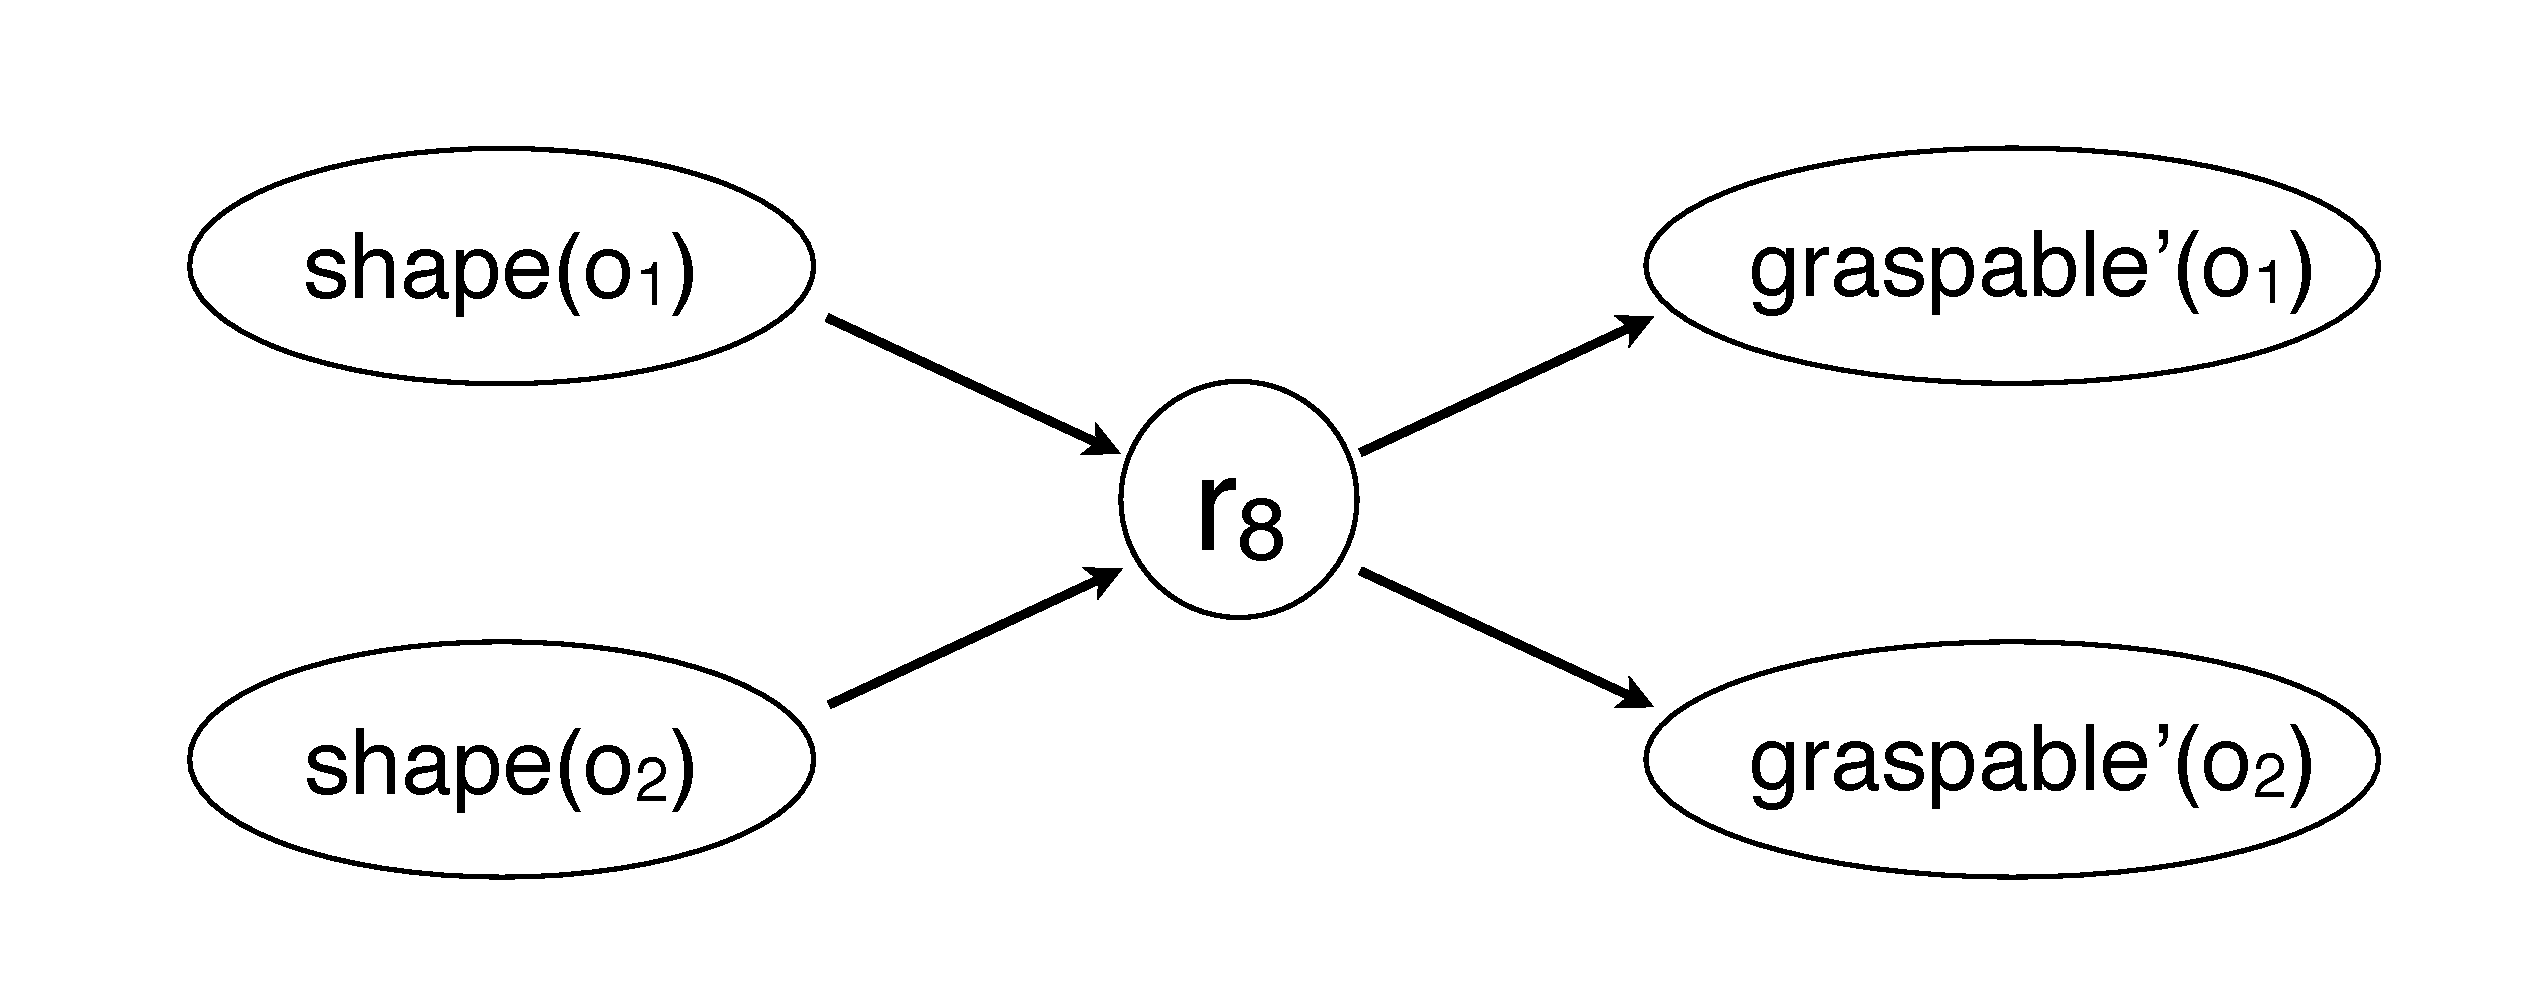
\includegraphics[scale=0.25]{imgs/quantruleinstantiation.pdf}
\caption{Instantiation of the quantified probability rule $r_8$ on a state with two objects $o_1$ and $o_2$.}
\label{fig:quantinstantitionprob}
\end{figure}

Given an input assignment such as $shape(o_1) = \mathit{spherical}$ and $shape(o_2) = \mathit{conic}$, the probability distribution $P(r_8 \, | \, \mathit{shape}(o_1)\!=\!\mathit{spherical}, \mathit{shape}(o_1)\!=\!\mathit{conic})$ that reflects the specification in the rule includes a total of four alternative effects: \begin{itemize}
\item $\{\mathit{graspable}(o_1)\!=\!true \land \mathit{graspable}(o_2)\!=\!true \} $ with probability $0.9 \times 0.2 = 0.18$ 
\item $\{\mathit{graspable}(o_1)\!=\!true \land \mathit{graspable}(o_2)\!=\!false\}$ with probability $0.9 \times 0.8 = 0.72$ 
\item $\{\mathit{graspable}(o_1)\!=\!false \land \mathit{graspable}(o_2)\!=\!true \}$ with probability $0.1 \times 0.2 = 0.02$ 
\item $\{\mathit{graspable}(o_1)\!=\!false \land \mathit{graspable}(o_2)\!=\!false\}$ with probability $0.1 \times 0.8 = 0.08$. 
\end{itemize}

We observe that the effects specified for $r_8$ mention two output variables: $\mathit{graspable}(o_1)$ and $\mathit{graspable}(o_1)$.  These two variables are therefore created as children of the node $r_8$. 

\subsubsection*{Utility distribution with quantifiers}

Rule-based utility distributions can be similarly extended to accommodate quantified variables. As for probability rules, quantified utility rules determine a set of groundings that satisfy at least one condition in the rule.  Each grounding $\mathbf{g}_k$ generates a particular utility distribution.  For a utility rule $r$ with input variables $I_1,...I_n$, decision variables $A_1,...A_m$ and quantified variables $\mathbf{x}$, one can find a set of groundings $G= \mathbf{g}_1,...\mathbf{g}_{|G|}$ that satisfy at least a condition. The total utility distribution is then defined by adding up the utility distributions for each grounding:

\begin{align}
& U_{r}(I_1\!=\!i_1,... I_n\!=\!i_n, A_1\!=\!a_1,... A_m\!=\!a_m) = \nonumber \\ 
&  \; \; \; \; \; \; \; \;  \sum_{k=1}^{|G|} U(D_i = \{A_1\!=\!a_1[\mathbf{g}_k / \mathbf{x}] \land... A_m\!=\!a_m[\mathbf{g}_k / \mathbf{x}]\}) \label{eq:quantifruledistrib}
 \\
& \; \; \; \; \; \; \; \; \text{where } i = \min_i (c_i[\mathbf{x} / \mathbf{g}_k]\text{ is satisfied with } I_1\!=\!i_1 \land ... I_n\!=\!i_n) \nonumber
\end{align}

Rule $r_9$ illustrates a simple utility rule that includes a quantified variable:
\begin{align*}
r_9: \ \ & \forall x: \\ 
& \textbf{if} \ (\mathit{graspable}(x) = \mathit{true})  \ \textbf{then} \\ 
& \;\;\;\;\; \begin{cases}
U(a_m\!=\!\mathit{grasp}(x)) = 2 \\
\end{cases} \\ 
&\textbf{else} \\ 
& \;\;\;\;\; \begin{cases}
U(a_m\!=\!\mathit{grasp}(x)) = -1 \\
\end{cases}
\end{align*}

The result of instantiating rule $r_9$ on a state with two objects $o_1$ with associated random variables $\mathit{graspable}(o_1)$ and $\mathit{graspable}(o_2)$ is shown in Figure \ref{fig:quantinstantitionutil}. 

\begin{figure}[h]
\centering
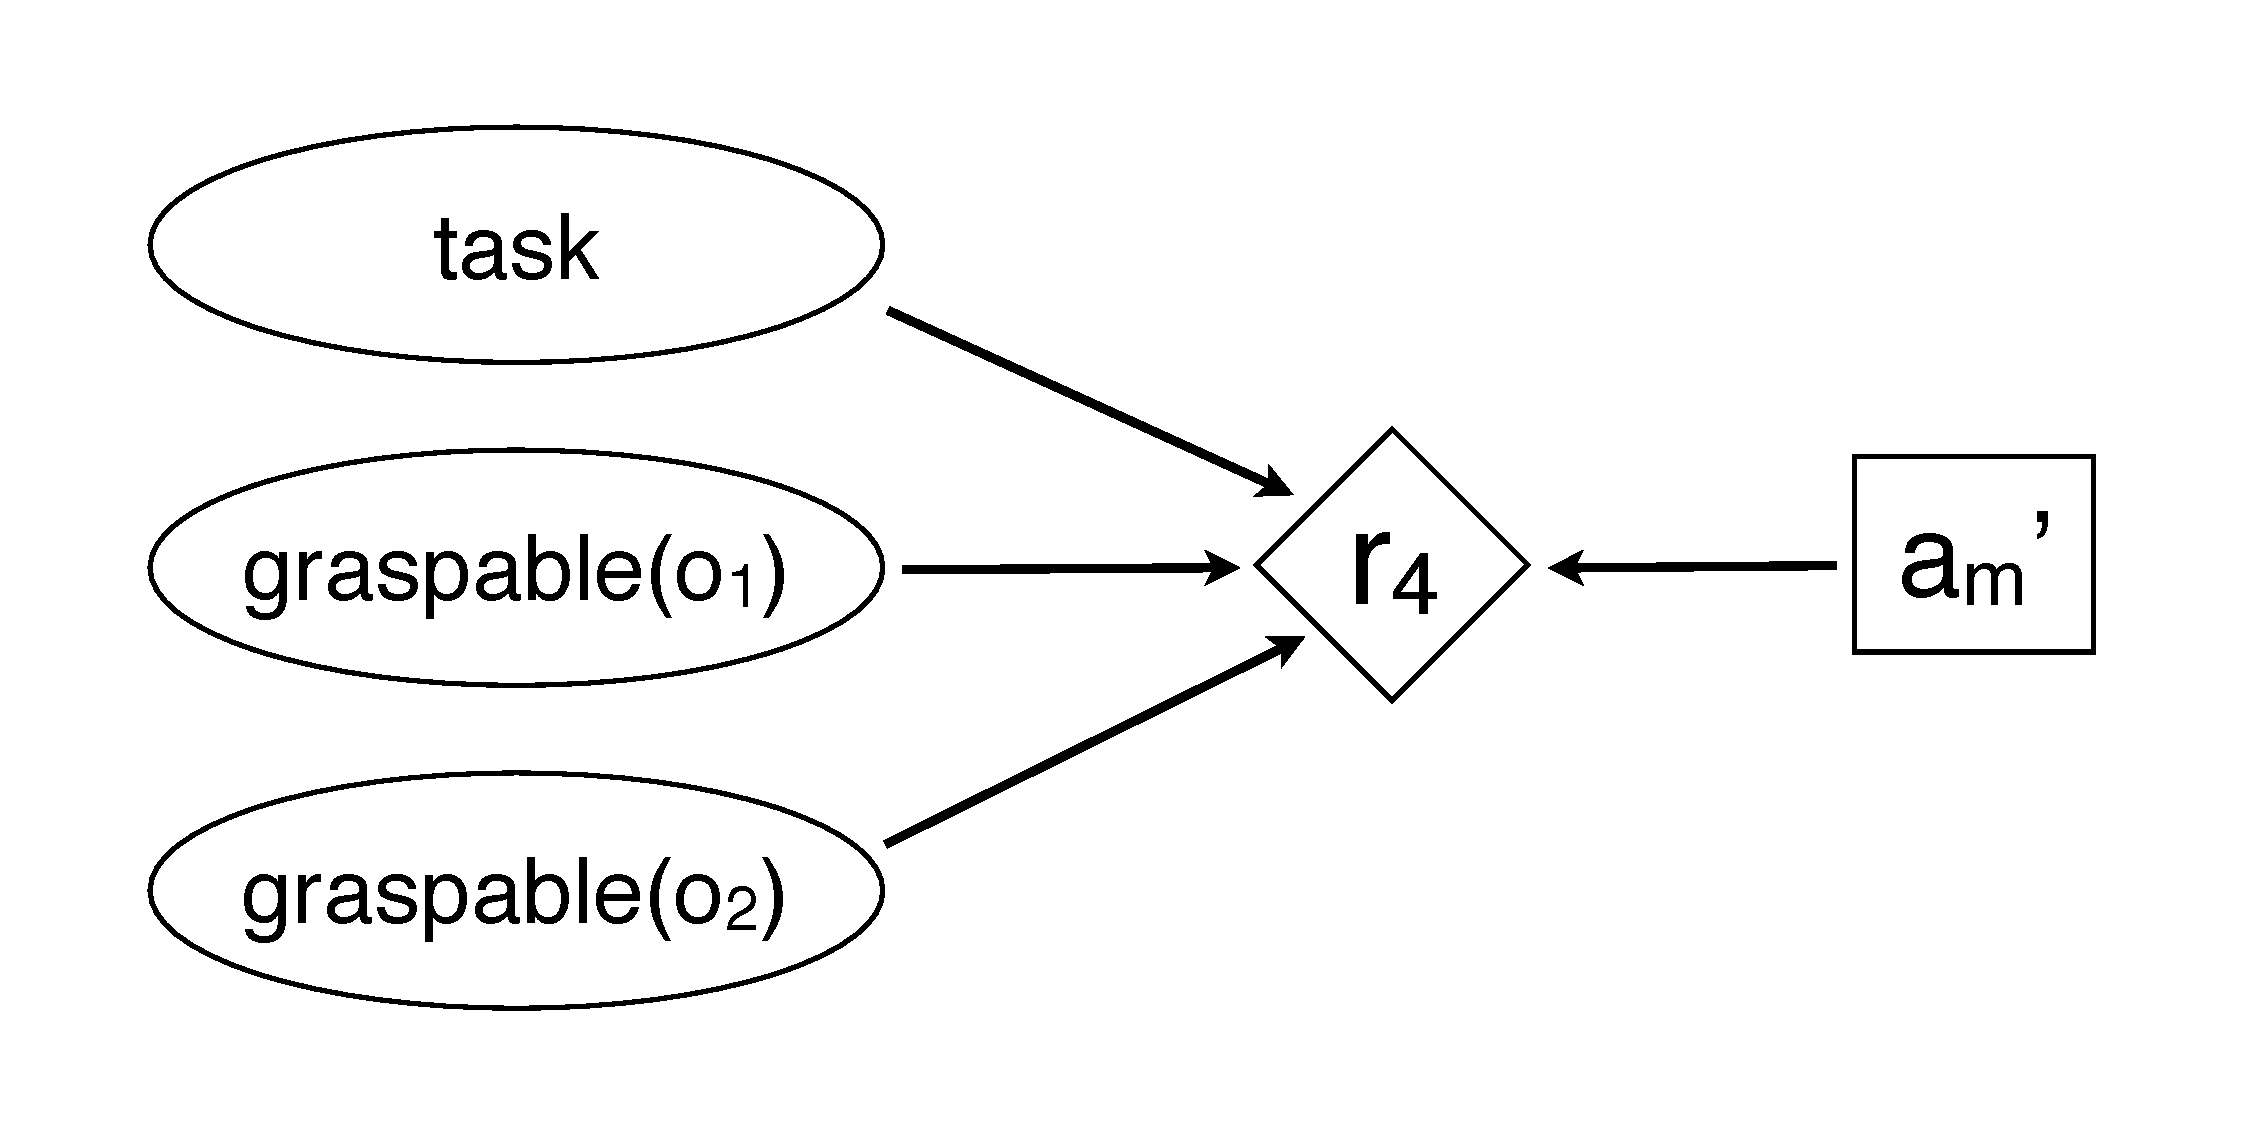
\includegraphics[scale=0.25]{imgs/quantutilruleinstantiation.pdf}
\caption{Instantiation of the quantified utility rule $r_9$ on a state with two objects $o_1$ and $o_2$.}
\label{fig:quantinstantitionutil}
\end{figure}

For a given input such as $\mathit{graspable}(o_1) = true \land \mathit{graspable}(o_2) = false$, two groundings $x=o_1$ and $x=o_2$ are found.  The total utility distribution is then straightforwardly derived to be:
\begin{itemize}
\item $U_r(\mathit{graspable}(o_1)\!=\!true, \mathit{graspable}(o_2)\!=\!false, a_m\!=\!\mathit{grasp}(o_1)) = 2$
\item $U_r(\mathit{graspable}(o_1)\!=\!true, \mathit{graspable}(o_2)\!=\!false, a_m\!=\!\mathit{grasp}(o_2)) = -1$
\end{itemize}

\section{Processing workflow}

The two previous sections have detailed how probability and utility rules are internally defined, and how they can be instantiated as nodes of a dynamic decision network. We are now ready to demonstrate how collections of rules can be applied to update the dialogue state and perform action selection. The general workflow is strongly inspired by information-state approaches to dialogue management \citep{Larsson:2000:ISD:973935.973943,Buckley:2006}, as the dialogue state serves as a central blackboard monitored by various groups of rules that are ``triggered'' upon relevant changes. 

We start by describing how the various rules describing a dialogue domain can be organised in collections called ``models''. We then show how these models are triggered to update state variables and express the utility of particular actions. We also demonstrate the general processing workflow on a detailed example. 


\subsection{Domain specification}

To ease the specification of dialogue domains, the probabilistic rules are grouped into collections called \textit{models}.  A model is simply a collection of rules that is associated with one or more ``trigger'' variables.  The update of such trigger variables in the dialogue state leads to the instantiation of all the rules included in the model. Formally, a model $m$ is defined as a pair $\langle \mathcal{T}_m, \mathcal{R}_m \rangle$ where $\mathcal{T}_m$ is a set of variables names that trigger the instantiation of the model, and $\mathcal{R}_m$ are the rules included in the model.

A dialogue domain is defined as a pair $\langle \mathcal{B}_0, \mathcal{M} \rangle$, where $\mathcal{B}_0$ is the initial dialogue state  and $\mathcal{M}$ the set of rule-based models attached to it. The organisation of rules into models allows the system designer to structure the application pipeline in a modular manner. Each model can be intuitively viewed as a distinct component responsible for a particular inference or decision step. Many reasoning tasks can be structured in terms of probabilistic rules.  Beyond the usual probability and utility models for dialogue management, probabilistic rules have also been applied to tasks related to natural language understanding and generation.  As an example, the dialogue domain specified for the experiments described in Chapter \ref{chap:user-evaluation} include a total of 6 models: one dialogue act classification model, (triggered by the user utterance $u_u$), one action utility model (triggered by the user dialogue act $a_u$), three probability models to predict the effects of the system action on the context, the user intention and the next user action (all triggered by the system action $a_m$), and a generation model (triggered by the system action $a_m$).  The association of trigger variables to the rule-based models provides a simple and flexible a way to define the processing pipeline for the application.  Variables can function as triggers for more than one model, allowing models to be instantiated in parallel.

As argued in \cite{lison-semdial2012}, the expressive power of probabilistic rules allow them to capture the structure of many dialogue processing tasks.  Compared to traditional architectures in which the components are developed separately and rely on ad hoc representation formats, the use of a shared formalism to encode the domain models yields several advantages:
\begin{description}
\item [Transparency: ] The reliance on a common representation format provides a unified, transparent semantics for the dialogue state, since all state variables are described and related to each other in a principled framework grounded in probabilistic inference.  This makes it possible to derive a semantic interpretation for the dialogue state as a whole (in terms e.g. of a joint probability distribution). 

\item [Domain portability: ]  As all domain-specific knowledge is declaratively specified in the rules, the system architecture is essentially reduced to a generic platform for rule instantiation and probabilistic inference.  This declarative design greatly enhances the system portability across domains, since adapting a system to a new domain only requires a rewrite or extension of the domain-specific rules, without having to reprogram a single component.  This stands in sharp contrast with ``black-box'' types of architectures where much of the task- and domain-specific knowledge is encoded in procedural form within the component workflow.

\item [Flexible workflow: ] Probability rules can design very flexible processing pipelines where state variables are allowed to depend or influence each other in any order and direction.  Models can be easily inserted or extended without requiring any change to the underlying platform. 

\item [Joint optimisation: ] Finally, the use of a unified modelling formalism allows the multiple domain models to be optimised jointly instead of tuning each model in isolation. Joint optimisation has recently gained much attention in the dialogue system community to overcome the fragmentation of current system architectures and attempt to directly optimise the end-to-end conversational behaviour of the system \citep{Lemon:2011}. 


\end{description}

\subsection{Update algorithm}

The software architecture adopted in this thesis takes the form of an event-driven, blackboard architecture \cite{Buckley:2006} revolving around a dialogue state $\mathcal{B}$ represented as a Bayesian network.  As in information state approaches, this dialogue state is read and written by the various modules integrated in the dialogue system. The general procedure to update the dialogue state upon the reception of new variables is provided in Algorithm \ref{algo:stateupdate}.
 
State update is performed whenever a chance occurs on one or more state variables, due to e.g. to new inputs processed by the ASR or NLU component. The first step of the algorithm is to incorporate the new variable in the dialogue state and possibly relate them to their predicted values (lines 2-3 of Algorithm \ref{algo:stateupdate}, see below for more explanation). The algorithm the triggers the instantiation of the relevant domain models (line 4), leading to a chain of updates.  If the expanded dialogue state contains decision and utility variables, the algorithms then searches for the optimal action, selects it, and activates the models that are triggered as a result of this action  (lines 6-8). Finally, outdated and intermediary nodes are pruned away from the expanded state and the evidence is incorporated in the state distribution (line 10). 

We now describe each of these steps in detail.

\begin{algorithm}[h]
\caption{: \textsc{UpdateState} ($\mathcal{B}, \mathbf{X}$)}
\begin{algorithmic}[1] \vspace{1mm}
\REQUIRE $\mathcal{B}$: Bayesian network for the current state
\REQUIRE $\mathbf{X}$: New random variables to insert in the state \vspace{1mm}
\STATE Initialise evidence $\mathbf{e} \leftarrow \emptyset$
\STATE Insert $\mathbf{X}'$ to the current state $\mathcal{B}$ 
\STATE $\mathcal{B}, \mathbf{e} \leftarrow $ \textsc{IntegratePredictions}($\mathcal{B}, \mathbf{e}, \mathbf{X}'$)
\STATE $\mathcal{B}, \mathbf{e} \leftarrow$ \textsc{TriggerModels} ($\mathcal{B}, \mathbf{e},  \mathbf{X}'$) \vspace{1mm}
\WHILE {$\mathcal{B}$ contains decision variables}
\STATE $\mathbf{a}^* \leftarrow $ \textsc{SelectAction} ($\mathcal{B}, \mathbf{e}$)
\STATE Assign $\mathbf{A}' = \mathbf{a}^*$
\STATE $\mathcal{B}, \mathbf{e} \leftarrow$ \textsc{TriggerModels} ($\mathcal{B}, \mathbf{e}, \mathbf{A}'$)
\ENDWHILE \vspace{1mm}
\STATE $\mathcal{B} \leftarrow \textsc{PruneState} (\mathcal{B}, \mathbf{e})$ \vspace{1mm}
\end{algorithmic}
\label{algo:stateupdate}
\end{algorithm}

\newpage
\subsubsection*{Connection between predictions and observations}


Some models are used to provide predictions on variables that will be observed in the next time steps.\footnote{This is notably the case for the user action model $P(a_u \, | \, i_u, a_m)$, which estimate the relative probabilities for the next dialogue action from the user. The prediction provide a prior on the future observation of the user action, and effectively prime the user actions that are most likely given a particular conversational situation.} In order to distinguish random variables that express a prediction on a future outcome from those that reflect an actual (although possibly uncertain) observation, we denote predictive variables in the dialogue state with a subscript $p$. A variable $X_p$ is thus a prediction for the future observation of the variable $X$. 

\begin{wrapfigure}[10]{r}{48mm}
\vspace{-6mm}
\centering
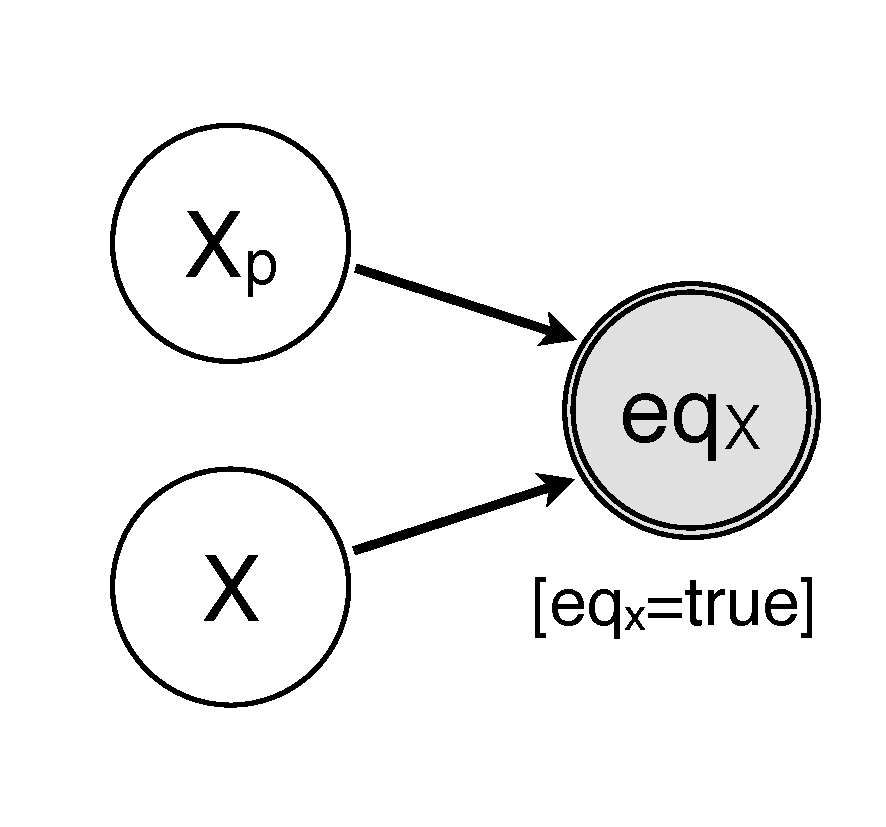
\includegraphics[scale=0.25]{imgs/prediction.pdf} 
\caption{Equivalence node $eq_{X}$ with parents $X$ and $X_p$.}
\label{fig:prediction}
\end{wrapfigure}

Prediction and observation variables must be connected with one another at runtime.  In the case where the observation is known with certainty, this connection can simply be represented as an assignment of evidence values.  However, dialogue domains often include observations that are themselves uncertain and must therefore rely on some type of soft evidence mechanism \citep{Pan06beliefupdate}.  The method adopted in this thesis is to add a new chance node, subsequently called the \textit{equivalence node} $eq_{X}$, with boolean values that is conditionally dependent on both $X$ and $X_p$.\footnote{The addition of a distinct node to express the evidence is necessary in our case since both $X$ and $X_p$ can have arbitrary incoming and outgoing edges with other variables in the dialogue state.}.  The conditional probability distribution of $eq_X$ is deterministic:
\begin{equation}
P(eq_{X}\!=\!true \, | \, X\!=\!x, X_p\!=\!x_p) = \begin{cases}
1 & \text{if } x = x_p \\
0 & \text{otherwise}
\end{cases} \label{eq:equivdistrib}
\end{equation}

The assignment $eq_{X} \!=\! true$ is added to the evidence. The posterior distribution given the evidence can then be straightforwardly derived to allow the prediction to act as a prior for the observed distribution.
\begin{align}
&P(X = x \, | eq_{X}\!=\!true) \nonumber \\
&=  \alpha \ P(X\!=\!x)  \sum_{x_p \in Val(X_p)} P(eq_{X}\!=\!true | X\!=\!x, X_p \!=\!x_p ) P(X_p\!=\!x_p) \\
&= \alpha \ P(X\!=\!x) \ P(X_p\!=\!x) \label{eq:equivalence}
\end{align}

Algorithm \ref{algo:integratepredictions} enumerates the steps involved in the integration of predicted values upon the update of the set of random variables $Vars$. 

\begin{algorithm}[h]
\caption{: \textsc{IntegratePredictions} ($\mathcal{B}, \mathbf{e}, Vars$)}
\begin{algorithmic}[1] \vspace{1mm}
\FORALL {$Var \in Vars$}
\IF {there is a corresponding prediction variable $Var_p \in \mathcal{B}$}
\STATE Create equivalence node $eq_{Var}$ with distribution in Eq. \eqref{eq:equivdistrib}
\STATE Insert $eq_{Var}$ in $\mathcal{B}$ with parents $\mathit{Var}$ and $\mathit{Var}_p$
\STATE Add assignment $[eq_{Var}\!=\!true]$ to evidence $\mathbf{e}$
\ENDIF
\ENDFOR
\RETURN $\mathcal{B}, \mathbf{e}$
\end{algorithmic}
\label{algo:integratepredictions}
\end{algorithm}


\subsubsection*{Model instantiation}

After inserting the new variables in the dialogue state and connecting them to their predicted values (if applicable), the next step is to trigger the relevant domain models . Algorithm \ref{algo:triggerModels} summarises the steps involved in the instantiation of the domain models following an update of the dialogue state. The algorithm takes three arguments: a dialogue state $\mathcal{B}$ represented as a Bayesian network, an assignment of evidence values and a list of random variables that have been recently updated in the dialogue state. The algorithm loops on all domain models and instantiates the ones that are triggered by the updated variables. Once all models are checked, the output variables of the instantiated rules become updated variables, and the procedure is repeated until no more model can be applied.  To avoid infinite triggering cycles, a model can only be instantiated once per update. 


\begin{algorithm}[h]
\caption{: \textsc{TriggerModels} ($\mathcal{B}, \mathbf{e}, \mathit{UpdatedVars}$)}
\begin{algorithmic}[1] \vspace{1mm}
\WHILE {$\mathit{UpdatedVars} \neq \emptyset$}
\STATE $\mathit{NewVars} \leftarrow \emptyset$
\FORALL {models $m$}
\IF {$\mathit{UpdatedVars} \cap \mathcal{T}_m \neq \emptyset$ and $m$ has not yet been applied}
\FORALL {rule $r \in \mathcal{R}_m$}
\IF {$r$ is a probability rule}
\STATE $\mathcal{B} \leftarrow \textsc{InstantiateProbRule}(\mathcal{B},r)$
\ELSIF {$r$ is a utility rule}
\STATE $\mathcal{B} \leftarrow \textsc{InstantiateUtilRule}(\mathcal{B},r)$
\ENDIF
\STATE Let $\mathcal{O}_r$ be the new output variables created by rule $r$
\STATE $\mathit{NewVars} \leftarrow \mathit{NewVars} \cup \mathcal{O}_r$
\STATE $\mathcal{B}, \mathbf{e} \leftarrow $ \textsc{IntegratePredictions}($\mathcal{B}, \mathbf{e}, \mathcal{O}_r)$
\ENDFOR
\ENDIF
\ENDFOR 
\STATE $\mathit{UpdatedVars} \leftarrow \mathit{NewVars}$
\ENDWHILE 
\RETURN $\mathcal{B}, \mathbf{e}$
\end{algorithmic}
\label{algo:triggerModels}
\end{algorithm}

\subsubsection*{Action selection}

If the dialogue state expanded with the instantiated rules contain utility and decision nodes, the system must in this case decide on the action to perform.  Algorithm \ref{algo:actionselection} illustrates how actions can be automatically selected on the basis of the current dialogue state augmented with decision and utility variables. The algorithm simply searches for the assignment of action values that maximise the current utility given the dialogue state and the evidence, and returns it. The utility nodes are removed from the state once the decision is made. Note that the action selection procedure shown in Algorithm \ref{algo:actionselection} only takes into account the current (immediate) utility and does not rely on any forward planning.  Chapter \ref{chap:rllearning} will demonstrate how this action selection mechanism can be expanded to perform online planning on a limited horizon. 

\begin{algorithm}[h]
\caption{: \textsc{SelectAction} ($\mathcal{B}, \mathbf{e}$)}
\begin{algorithmic}[1] \vspace{1mm}
\STATE Let $\mathbf{A}'$ be the set of all decision variables in $\mathcal{B}$
\STATE Find optimal value $\mathbf{a}^* = \argmax_{\mathbf{a}} U(\mathbf{A}' = \mathbf{a}, \mathbf{e})$
\STATE Remove utility nodes from the state $\mathcal{B}$
\RETURN $\mathbf{a}^*$
\end{algorithmic}
\label{algo:actionselection}
\end{algorithm}


\subsubsection*{State pruning}

The instantiation of the domain models in the dialogue state results in the integration of multiple new nodes in the dialogue state. This monotonic expansion of the dialogue state may quickly lead to tractability problems if left unchecked.  The last step of state update is therefore to reduce the dialogue state to its minimal size, by removing all intermediary nodes -- such as rule nodes, outdated versions of state variables, equivalence nodes and predictive nodes that are attached to them -- in order to only retain current state variables. The accumulated evidence attached to the equivalence nodes is also integrated in the posterior distribution of the state variables.

The procedure is outlined in Algorithm \ref{algo:pruneState}. The first step is to determine which nodes to keep (line 1-6).  Only the most recent versions of state variables are retained. 
The nodes are then added one by one in a new dialogue state $\mathcal{B}'$.  The parents of each variable is determined, and its conditional probability distribution is calculated given the evidence.  The parents of a state variable are the closest ancestors of the variable in the set of nodes to keep. 


\begin{algorithm}[h]
\caption{: \textsc{PruneState} ($\mathcal{B}, \mathbf{e}$)}
\begin{algorithmic}[1] \vspace{1mm}
\STATE $\mathit{NodesToKeep} \leftarrow \emptyset$
\FORALL {node $N \in \mathcal{B}$}
\IF {$N$ is a state variable and $\nexists \ N' \in \mathcal{B}$}
\STATE $\mathit{NodesToKeep} \leftarrow \mathit{NodesToKeep} \cup [N]$ 
\ENDIF
\ENDFOR
\STATE Create new state $\mathcal{B'} \leftarrow \emptyset$
\FORALL {node $N \in  \mathit{NodesToKeep}$}
\STATE Add node $N$ to $\mathcal{B'}$ (with primes removed from node name)
\STATE $\mathit{Parents} \leftarrow \{M \in \mathit{NodesToKeep} : M \text{ is an ancestor of } N \text{ and there is } $ \\ $\phantom{a}$  \; \; \; \; \; \; \; \; \;  a path $M \rightarrow^+  N \text{ without node in } \mathit{NodesToKeep} \}$ 
\STATE Add dependency edges between $\mathit{Parents}$ and $N$ in $\mathcal{B}'$
\STATE Assign distributions $P_{\mathcal{B}'}(N \, | \, \mathit{Parents}) \leftarrow P_{\mathcal{B}}(N \, | \, \mathit{Parents}, \mathbf{e})$
\ENDFOR
\RETURN $\mathcal{B}'$
\end{algorithmic}
\label{algo:pruneState}
\end{algorithm}


Figure \ref{fig:pruning} illustrates the input and output of the pruning process.  Only the nodes $A'$, $B$, $C$, $D$ and $E'$ are retained. Note that that the primes are deleted from the random variable names.

\begin{figure}[h]
\centering
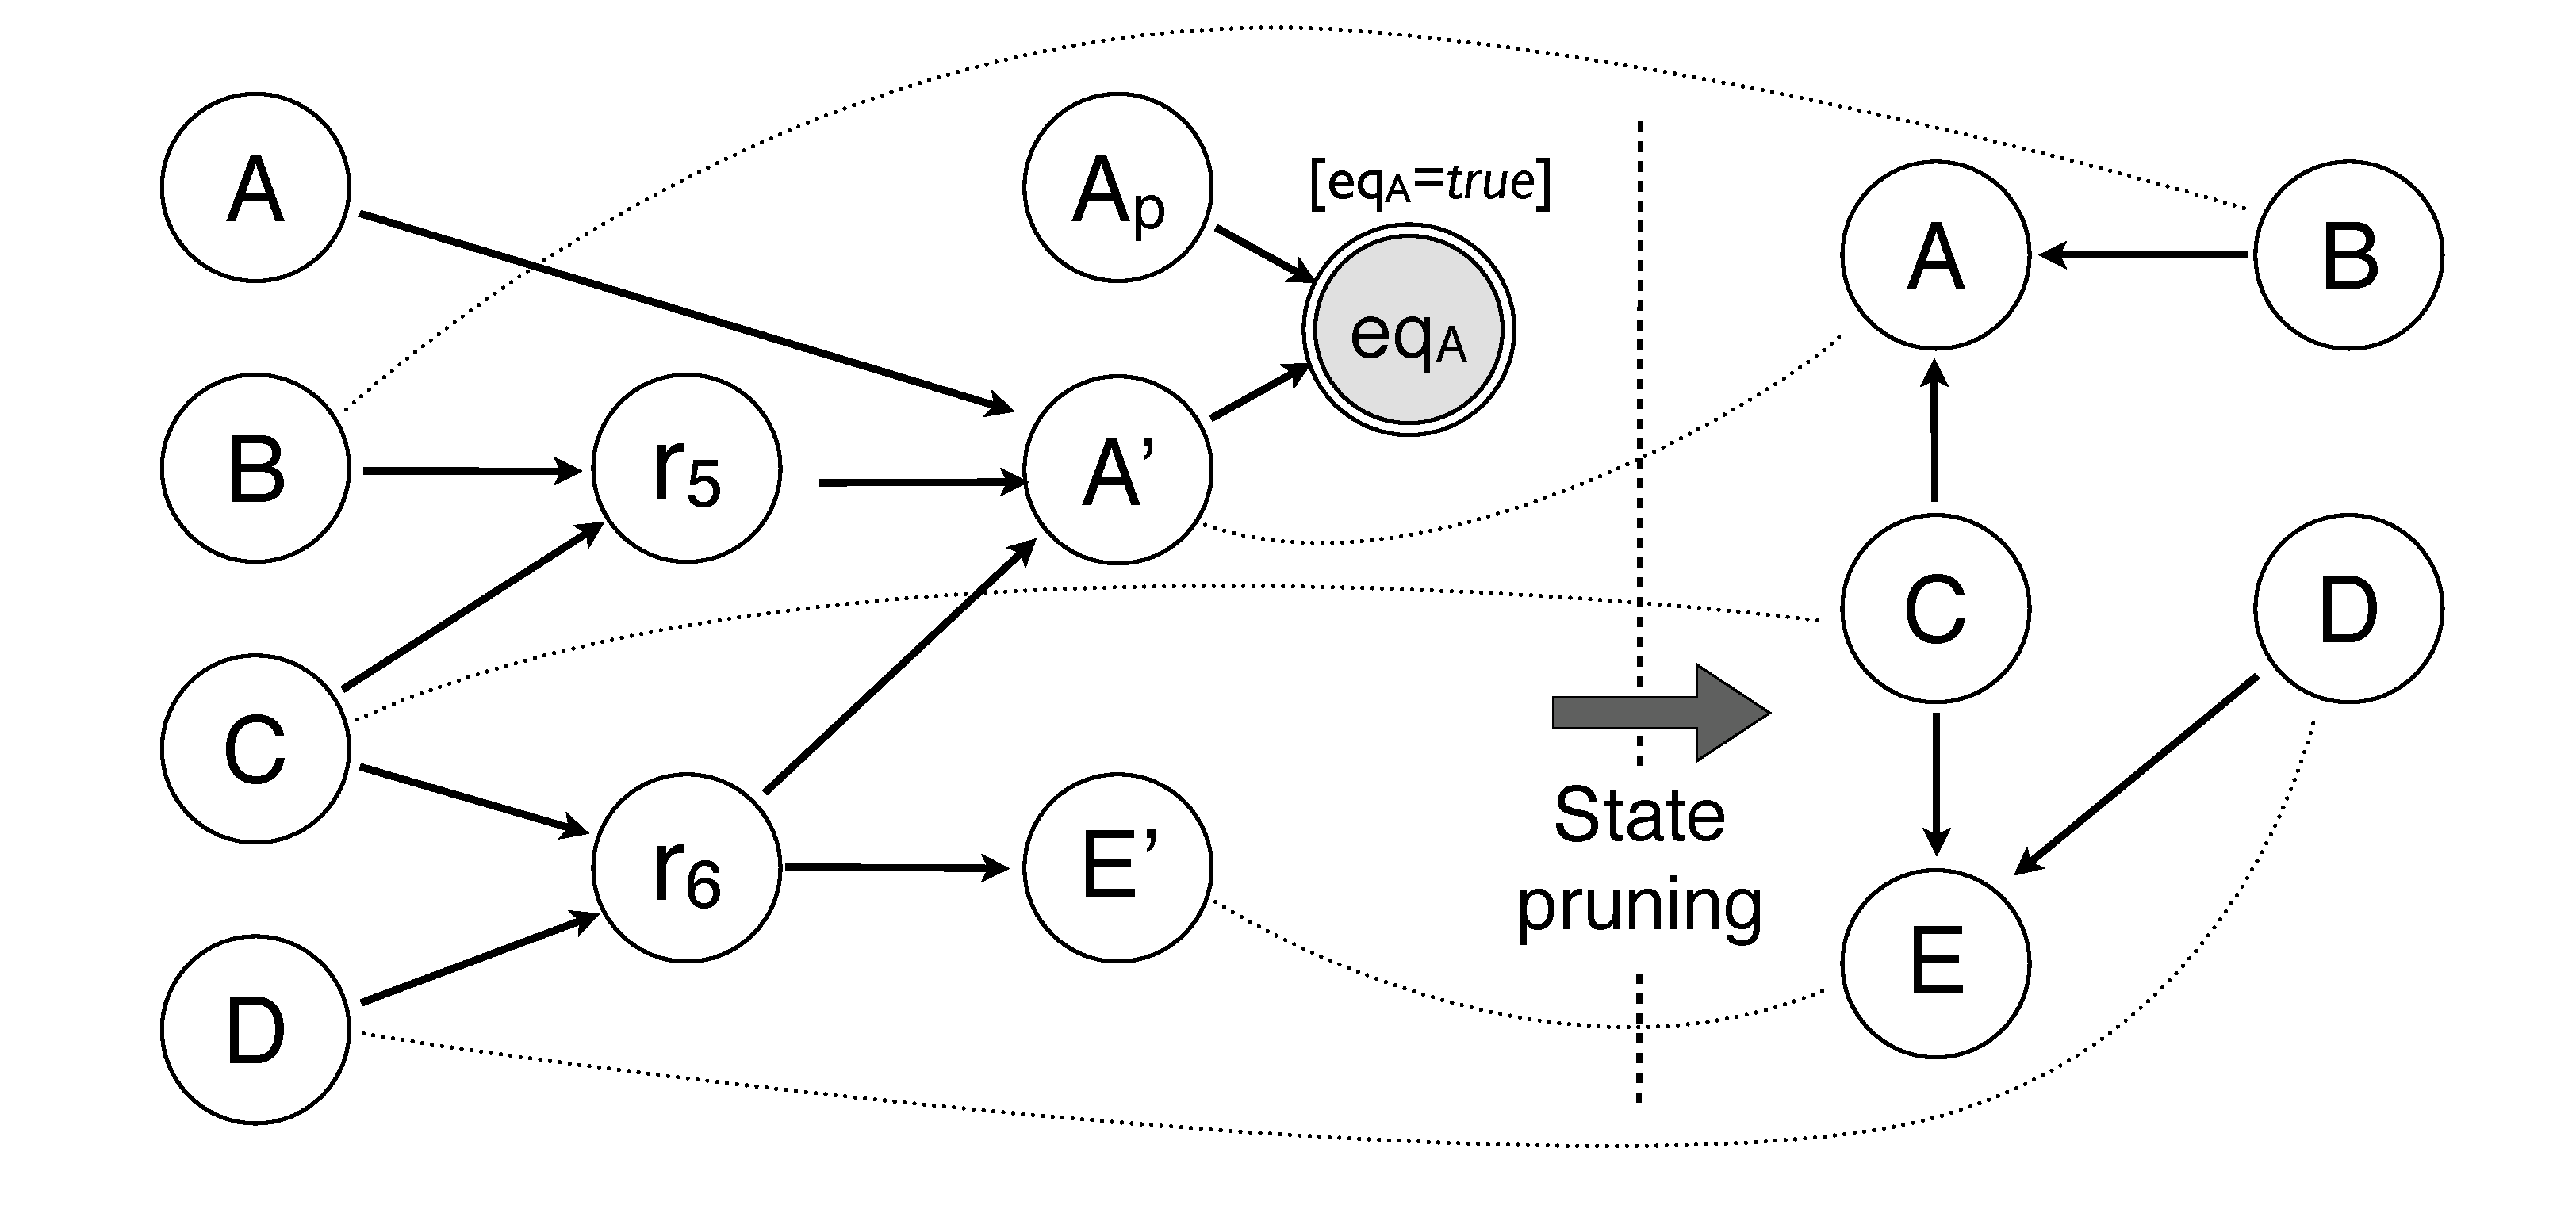
\includegraphics[scale=0.20]{imgs/pruning.pdf}
\caption{Illustration of the state pruning process. The left side shows a dialogue state before pruning, and the right side the corresponding state following the pruning operation. The dotted lines denote the correspondence between nodes.}
\label{fig:pruning}
\end{figure}


\subsection{Detailed example}

\subsubsection*{Description}

Assume a domain similar to the one shown in Figure \ref{fig:fsa}, where a user can request a robot to move forward, backward, left, right, or stop.  The set of dialogue acts $a_u$ that can be recognised by the system is the following: 
\begin{center}
$\{\mathit{Request(Forward)}$, $\mathit{Request(Backward)}$, $\mathit{Request(Left)}$, \\ $\mathit{Request(Right)}$, $\mathit{Request(Stop)}$, $\mathit{Other}\}$. \\
\end{center}
The corresponding system actions $a_m$ are: 
\begin{center}
$\{\mathit{Move(Forward)}$, $\mathit{Move(Backward)}$, $\mathit{Move(Left)}$, \\ $\mathit{Move(Right)}$, $\mathit{Move(Stop)}$, $\mathit{AskRepeat}\}$. 
\end{center}
The objective of the system is to fulfil the user command if it is reasonably certain of which action to execute.  Otherwise, the system asks the user to repeat. 

\subsubsection*{Domain specification}

The domain specification designed for this constructed example is constituted of an empty initial state and the following two rule-based models: \begin{description}
\item[Model $m_1$: ] Model $m_1$ is triggered by $a_u$ and includes two utility rules $r_{10}$ and $r_{11}$:
\begin{align*}
r_{10}: \ \ & \forall x: \\ 
& \textbf{if} \ (a_u = Request(x)) \ \textbf{then} \\ 
& \begin{cases} 
U(a_m = Move(x)) = 2 \\ 
\end{cases} \\
& \textbf{else} \\ 
& \begin{cases} 
U(a_m = Move(x)) = -2 \\ 
\end{cases} \\[4mm]
r_{11}: \ \ &  \begin{cases} U(a_m = \mathit{AskRepeat}) = 0.5 \end{cases}
\end{align*}

Rule $r_{10}$ specifies that the utility of executing the action corresponding to the user command is 2, with a penalty of $-2$ when the wrong action is executed. Rule $r_{11}$ assign a utility of 0.5 for asking a clarification question.  

\item[Model $m_2$: ] Model $m_2$ is triggered by $a_m$ and includes the predictive rule $r_{12}$: 
\begin{align*}
r_{12}: \ \ & \forall x: \\ 
& \textbf{if} \ (a_m = \mathit{AskRepeat} \land a_u=x) \ \textbf{then} \\ 
& \begin{cases} 
P(a_{u-p} = x) = 0.9 \\ 
\end{cases}
\end{align*}
Rule $r_{12}$ specifies that the probability that the user will repeat his last utterance when asked by the system to do so amounts to $0.9$.
\end{description}

\subsubsection*{Processing workflow}

Figure \ref{fig:detailedexample} details the steps involved in the state update after receiving dialogue act hypotheses from the natural language understanding component. The example covers the following short interaction: 
\begin{dialogue} 
\speak{User } Now move forward 
\speak{$\tilde{a}_u$} $\langle $(\textit{MoveForward}, 0.6), (\textit{MoveBackward}), 0.4)$\rangle$
\speak{System } Could you please repeat?
\speak{User } Please move forward!
\speak{$\tilde{a}_u$} $\langle $(\textit{MoveForward}, 0.7), (\textit{MoveLeft}, 0.2), (\textit{MoveBackward}, 0.1) $\rangle$
\speak{System } OK, moving forward!
\end{dialogue}


\begin{figure}[p]
\centering
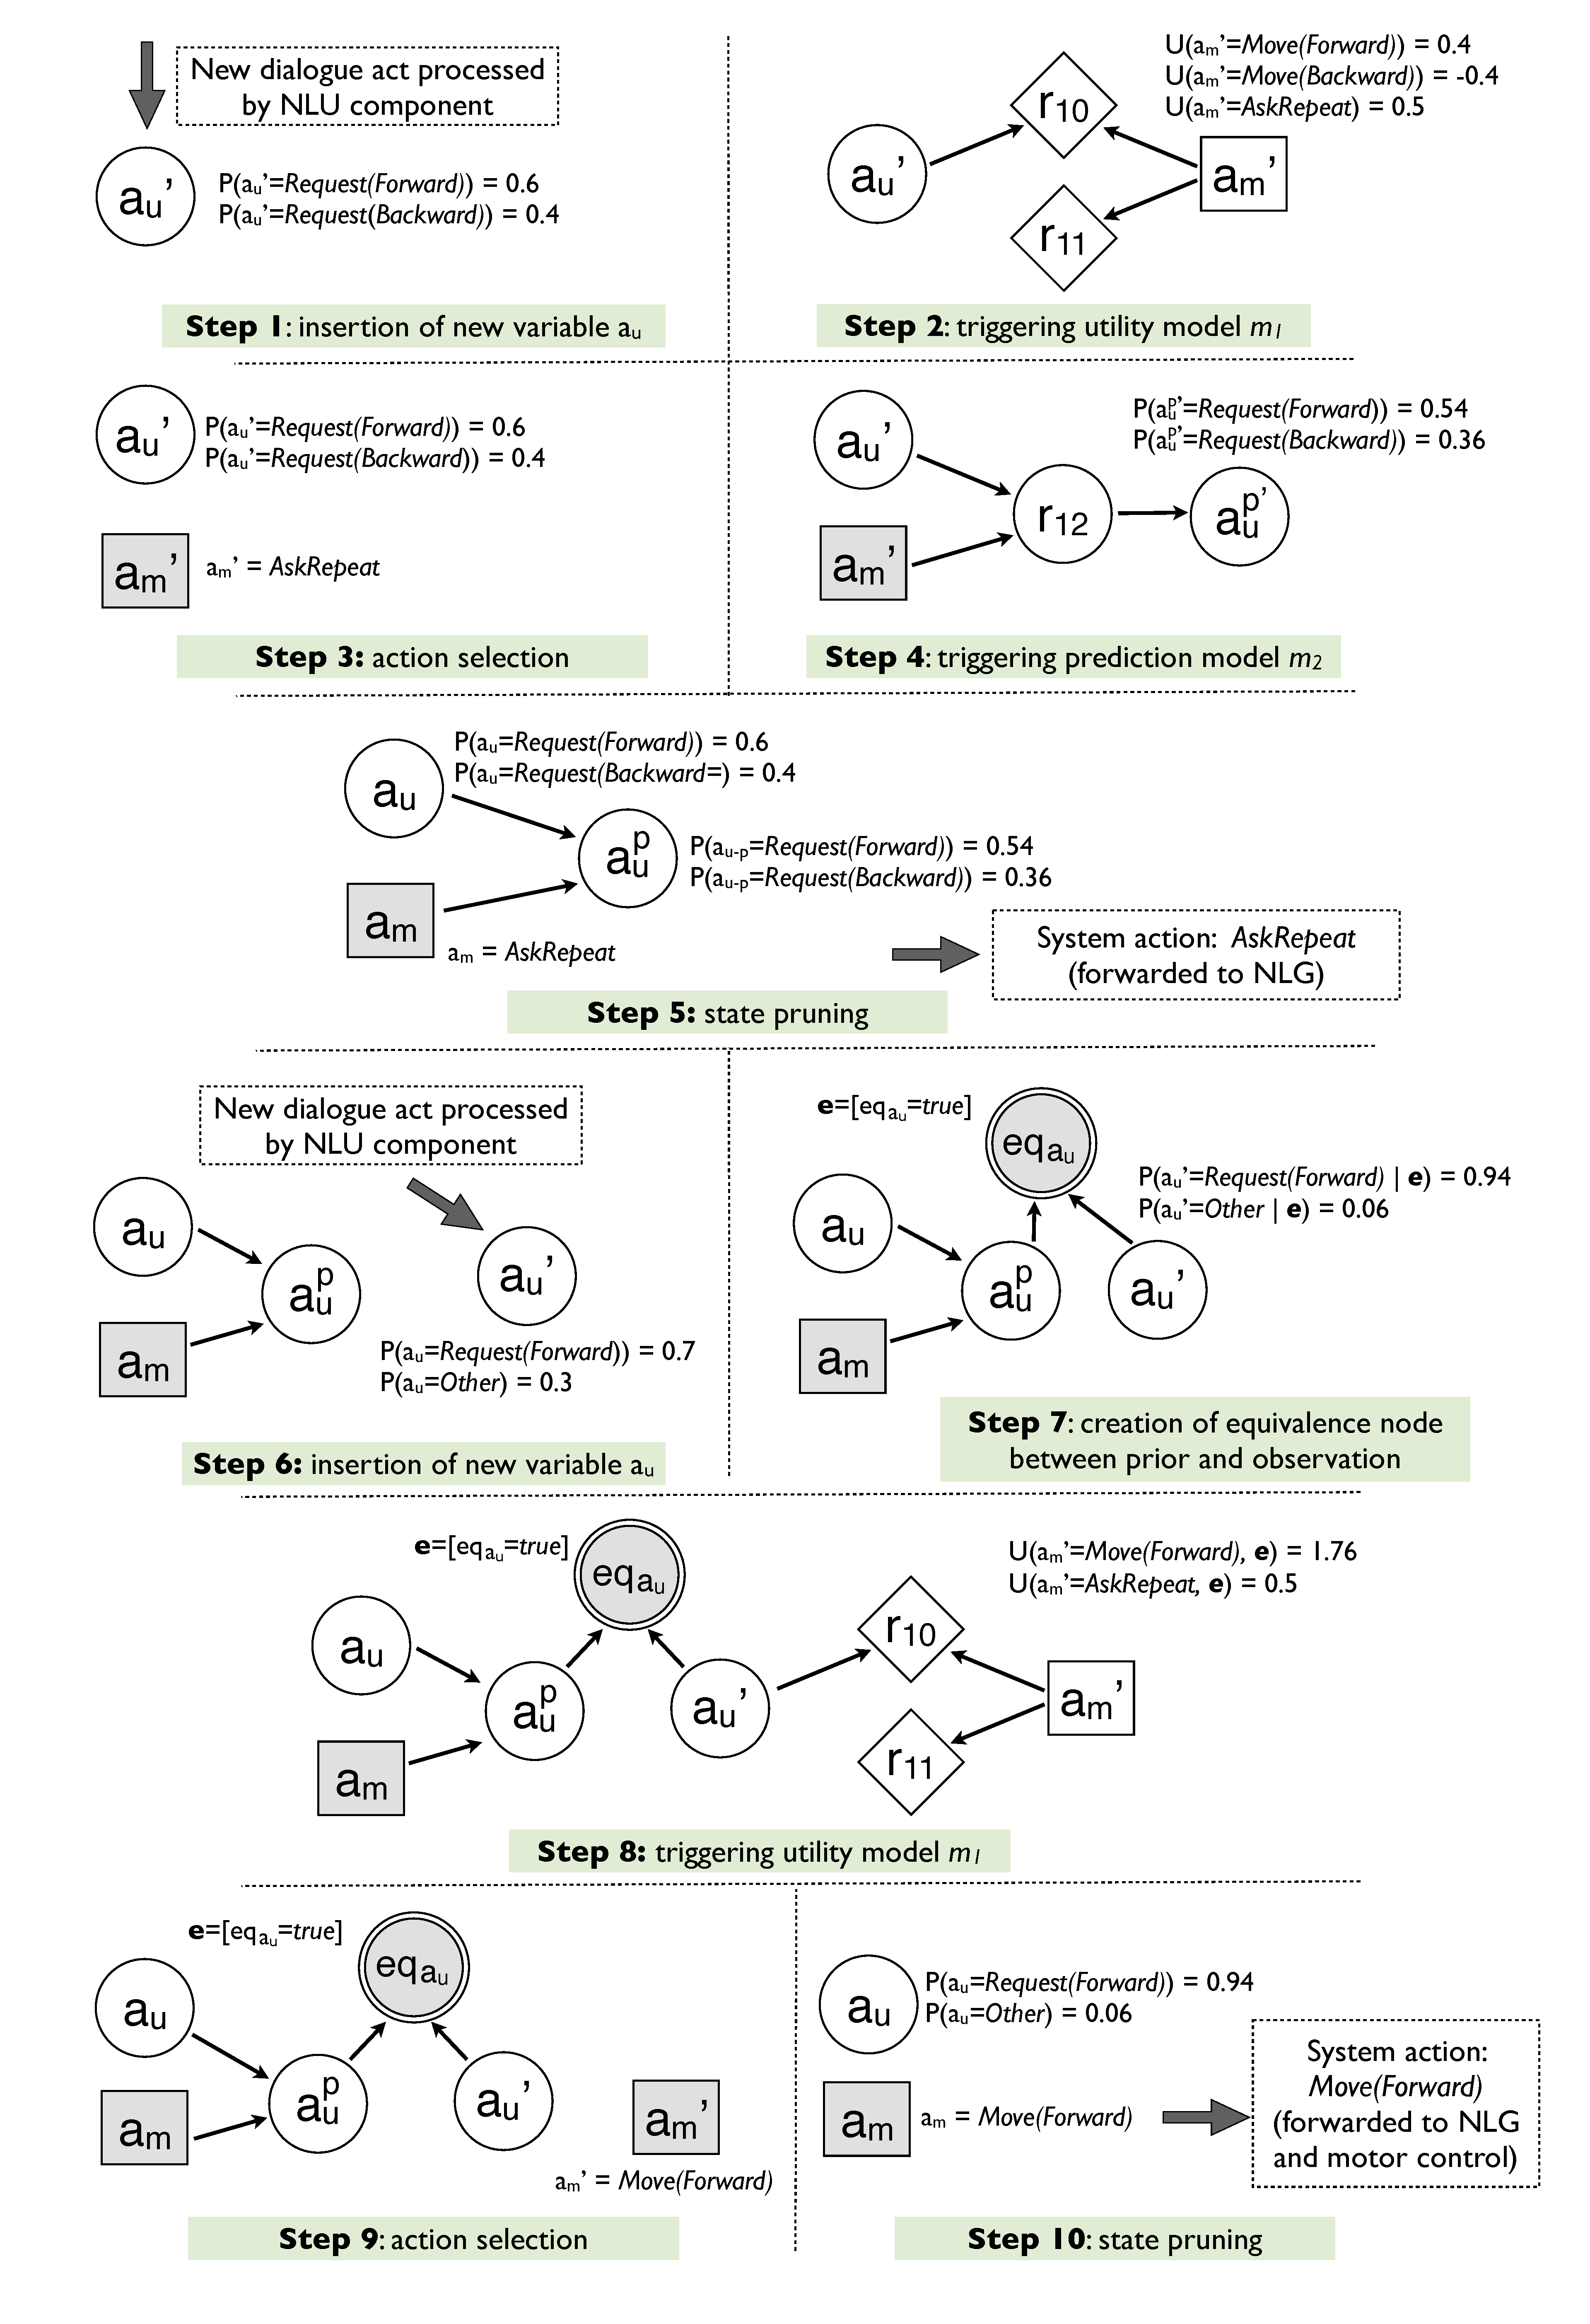
\includegraphics[scale=0.25]{imgs/detailedexample.pdf}
\caption{Detailed example of processing workflow. }
\label{fig:detailedexample}
\end{figure}
 
 
Step 1 inserts the new dialogue act hypotheses on the dialogue state.  This insertion triggers 
model $m_1$ since the model contains $a_u$ as trigger variable. The model instantiation results in Step 2 in the creation of two utility nodes and one decision node.  The optimal action to perform in such case is $\mathit{AskRepeat}$, which is selected by the system in Step 3. The action selection triggers model $m_2$ in Step 4, which creates a prediction node $a_{u-p}'$ expressing the expected values for the next user dialogue act. The state is finally pruned of the intermediary rule node in Step 5.  System components such as NLG can react on the updated state and generate the proper linguistic realisation of the system action. The system then waits for the user input, which is shown in Step 6.  The relation between the predicted and actual user response leads in Step 7 to the creation of an equivalence node, and the inclusion of the assignment $eq_{a_u} = true$ in the evidence. We notice that the combination of the prior distribution over predicted values and the actual distribution over dialogue act hypotheses increases the probability of $a_u' = \mathit{Request(Forward)}$. Step 8 triggers the model $m_1$ based on the new user input.  The optimal action is this case is $\mathit{Move(Forward)}$, which is selected in Step 9.  The model $m_2$ is triggered upon this selection but rule $r_{12}$ only generates an empty effect and is therefore directly deleted. Finally, the state is pruned of its intermediary nodes in Step 10, leaving only the last user and system actions $a_u$ and $a_m$. 


\section{Advanced modelling}
\label{sec:amodelling}

Dialogue domains often need to represent random variables whose values are expressed via specific data structures such as collections or strings. The rule-based formalism described in the previous sections must be extended to efficiently operate on these data structures.  We first describe how conditions and effects can be defined on variables that represent collections, and then discuss how rules can manipulate strings. 

\subsection{Operations on collections}

Some state variables are best represented as collections of elements. For instance, the dialogue state may include variables that enumerate e.g. the $n$ most recent dialogue acts in the interaction history, the stack of tasks that remain to perform, or the list of visual objects perceived by the system.  The range of values for such state variables is the power set of the set of possible elements. 

Both the conditions and effects of probabilistic rules can be adapted to include special-purpose operations for collections:
\begin{itemize}
\item Rule conditions can include checks on the presence or absence of particular elements in a collection, such as $a \in A$ or $a \notin A$. 
\item Rule effects can also be augmented to manipulate elements from a collection.  Three new types of effects are created to this end, in addition to the traditional assignment of output values: \textit{add effects} (adding an element to a collection), \textit{remove effects} (deleting an element from a collection) and \textit{clear effects} (clearing all elements of a collection). The resulting collections are sorted by insertion order. 
\end{itemize}

Figure \ref{fig:seteffects} illustrates two rules that make use of add and remove effects to update the distribution defined for the state variable $A$. 
 
\begin{figure}[h]
\centering
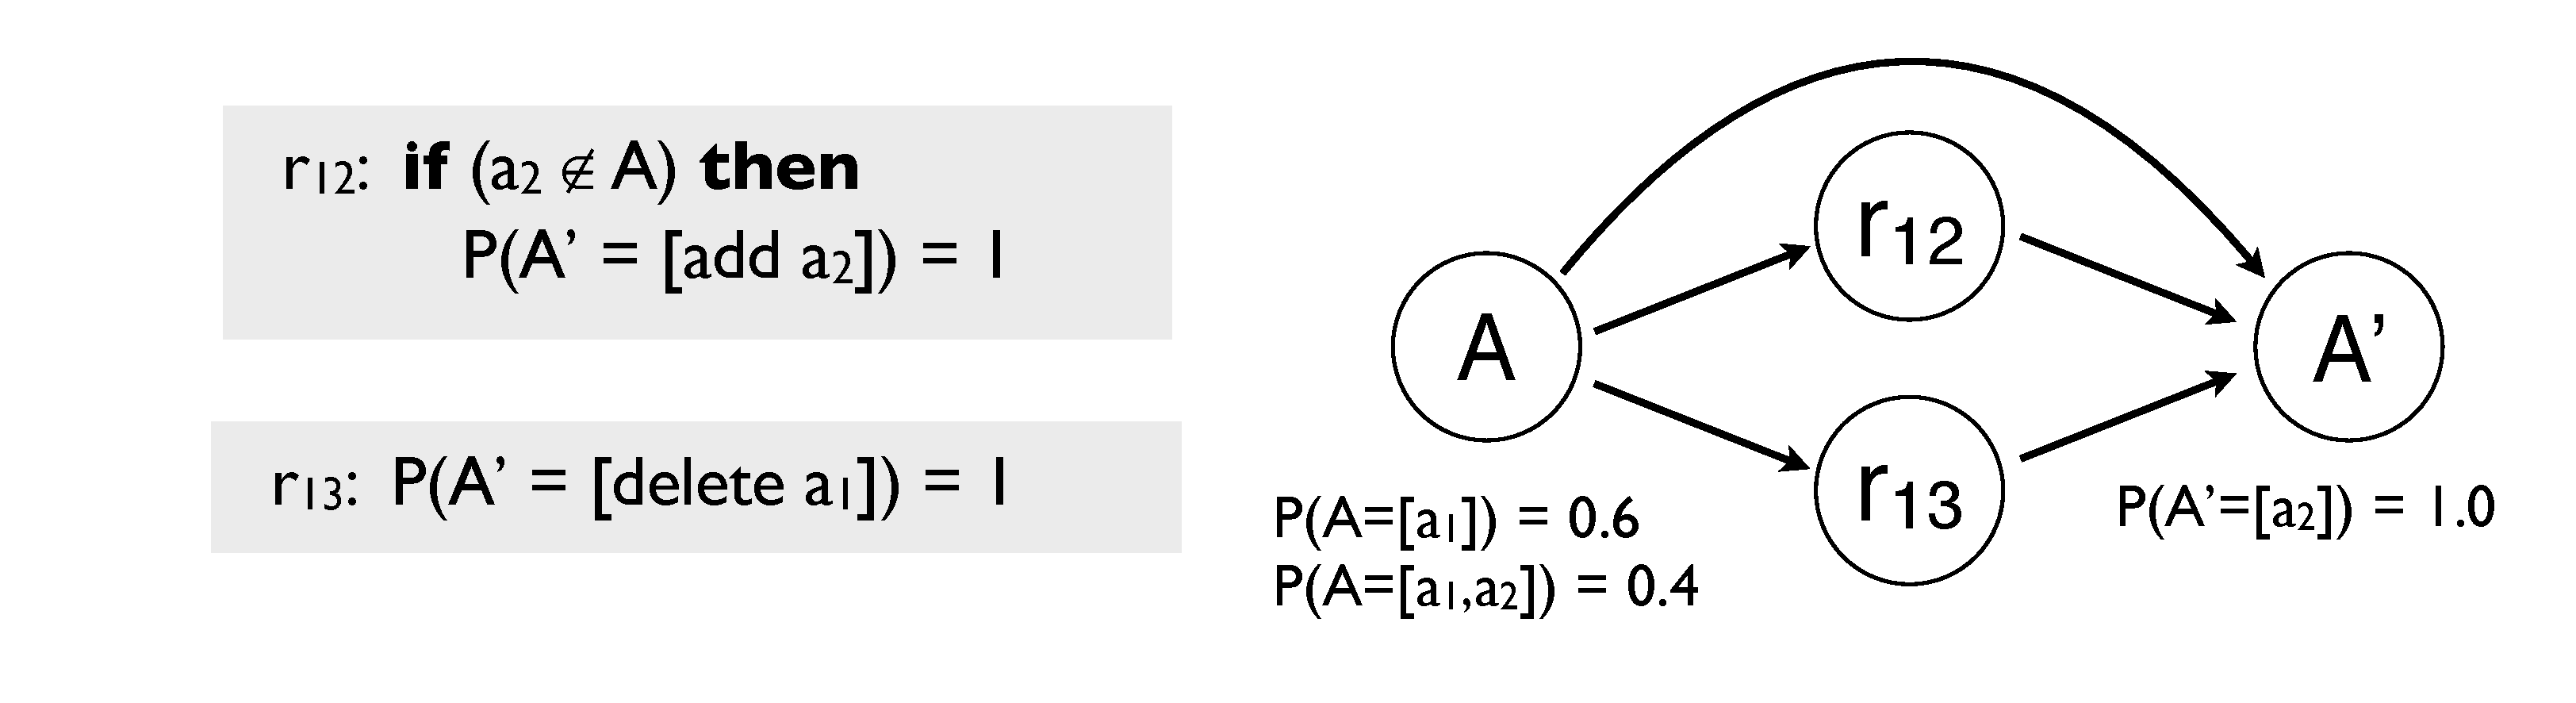
\includegraphics[scale=0.25]{imgs/seteffects.pdf}
\caption{Example of rules using add/remove effects to manipulate collections.}
\label{fig:seteffects}
\end{figure}


Output distributions $P(X'\!=\!x' \, | \, r_1\!=\!e_1,... r_n\!=\!e_n)$ must be adapted to take into account the three types of effects.  Let $\mathbf{e}$ denote as before the conjunction of all effects $e_1 \land ... e_n$. In addition to the classical set of values $\mathbf{e}(X)$ assigned for the variable $X$, the distribution also refers to the set of values $\mathbf{e}_{add}(X)$ and $\mathbf{e}_{remove}(X)$ that are to be respectively added and removed from the variable $X$.  A boolean  $\mathbf{e}_{clear}(X)$ indicates whether at least an effect requires the existing values for $X$ to be cleared.

Given these definitions, the output distribution defined in Equation \eqref{eq:outputdist1} for a new output variable can then be rewritten as: 
\begin{align}
&P(X'\!=\!x' \, | \, r_1\!=\!e_1,... r_n\!=\!e_n) = \hspace{10cm} \nonumber \\ & \; \; \; \; \; \begin{dcases} 
\frac{\sum_{v \in {\mathbf{e}(X)}} \mathbf{1}(x' = v)} { |\mathbf{e}(X)| }&  \text{if } \mathbf{e}(X)\!\neq\!\emptyset \\
\mathbf{1}(x' = \mathbf{e}_{add}(X))  &  \text{if } \mathbf{e}(X)\!=\!\emptyset \ \text{ and } \ \mathbf{e}_{add}(X)\!\neq\!\emptyset \\
\mathbf{1}(x' = \mathit{None}) & \text{otherwise}
\end{dcases}\label{eq:outputdist3}
\end{align}

The traditional assignment effects in $\mathbf{e}(X)$ and the add effects $\mathbf{e}_{add}(X)$ are mutually incompatible (in case both $\mathbf{e}(X)$ and $\mathbf{e}_{add}(X)$ are non-empty, the assignment effects are by convention assumed to take precedence). 

In case the output variable replaces an existing variable, the output distribution becomes:
\begin{align}
&P(X'\!=\!x' \, | \, r_1\!=\!e_1,... r_n\!=\!e_n, X\!=\!x) = \hspace{10cm} \nonumber \\ & \; \; \; \; \;  \begin{dcases} 
\frac{\sum_{v \in {\mathbf{e}(X)}} \mathbf{1}(x' = v)} { |\mathbf{e}(X)| }  & \text{if } \mathbf{e}(X)\!\neq\!\emptyset \\
\mathbf{1}(x' = \left[\mathbf{e}_{add}(X) \cup \left[x \ \backslash \ \mathbf{e}_{remove}(X)\right]\right]) & \text{if } \mathbf{e}(X)\!=\!\emptyset \ \text{ and } \ \neg \ \mathbf{e}_{clear}(X) \\
\mathbf{1}(x' = \mathbf{e}_{add}(X))  &  \text{if } \mathbf{e}(X)\!=\!\emptyset, \mathbf{e}_{add}(X)\!\neq\!\emptyset \ \text{ and }  \mathbf{e}_{clear}(X) \\
\mathbf{1}(x' = \mathit{None}) & \text{otherwise}
\end{dcases}\label{eq:outputdist4}
\end{align}


\subsection{Operations on strings}

Many of the data structures present in the dialogue state are strings -- including for instance the user utterance $u_u$ and the system utterance $u_m$. It is therefore useful to provide special-purpose functionalities for manipulating strings within the conditions and effects of probabilistic rules. In particular, rules can be extended to perform template-based string matching operations.  The idea is to include a new type of conditions that checks whether a string matches a given template.  Both full and partial matching can be employed. The template can include slots to fill, and the values extracted for these slots can be locally reused in the effects of the rule.  

Figure \ref{fig:stringmanip} illustrate how such rule are applied in practice.  $\{OBJ\}$ denotes a slot that is to be filled through matching the template with the value specified in $u_u$. 
\begin{figure}[h]
\centering
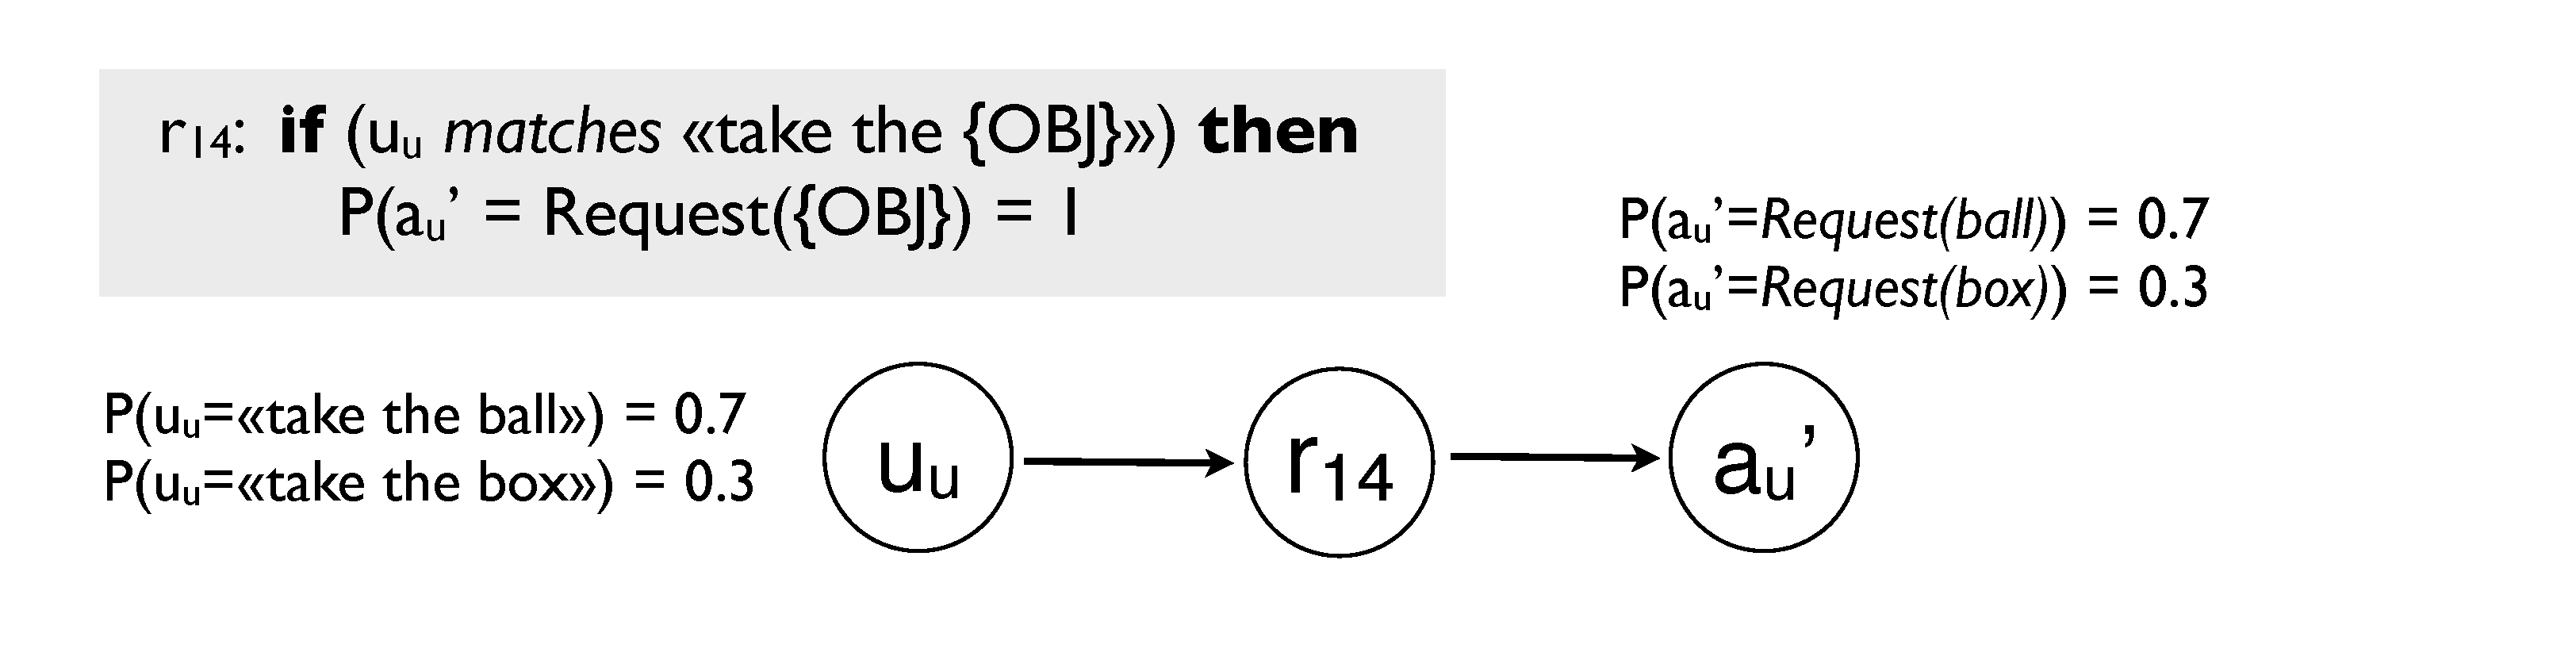
\includegraphics[scale=0.25]{imgs/stringmanip.pdf}
\caption{Example of rule using string matching operations.}
\label{fig:stringmanip}
\end{figure}

Such string matching functionality can be accommodated by adapting the rule distribution in Equation \eqref{eq:ruledistrib} in the following manner: 
\begin{align}
& P(r\!=\!e \, | \, I_1\!=\!i_1,... I_n\!=\!i_n) = P(E_i = e[\mathbf{s}_i\backslash \mathbf{x_i}]) \label{eq:ruledistribstring}
 \\ 
& \; \; \; \; \; \; \; \; \text{ where } i = \min_i (c_i \text{ is satisfied with } I_1\!=\!i_1 \land ... I_n\!=\!i_n) \text{ with filled slots } \mathbf{s}_i \nonumber 
\end{align}

The careful reader may notice that the above equation is similar to the rule distribution for quantified rules, with the exception that only one ``grounding'' (corresponding here to the filled slots) is extracted for a given input assignment.

\section{Related work}
\label{sec:relatedwork}

\note{Heriberto's relational state: \cite{pub5502} an hierarchical aproach \citep{Heriberto2011}}. 

\note{Otterlo2012}

\note{parameter sharing}

\note{ref to reinforcement learning based on same idea of if then else lists}

\note{link with PDDL, PPDDL, RPDDL!}

\note{incrementality!}

\section{Conclusion}

\note{way to structure a dynamic decision network, hence a POMDP}

